% =====================================================================
%  07-Compilers-Parser-SDT.tex
%  Technical report - Parser & SDT (Syntax and Semantic Analyzer)
%  Team 07 - Compilers, Group 5 - Faculty of Engineering, UNAM
% =====================================================================
\documentclass[11pt,letterpaper]{article}

\usepackage[utf8]{inputenc}
\usepackage[T1]{fontenc}
\usepackage[english]{babel}
\usepackage{lmodern}
\usepackage[margin=2.5cm]{geometry}
\usepackage{amsmath,amssymb}
\usepackage{booktabs,array,tabularx,longtable}
\usepackage{xcolor}
\usepackage{listings}
\usepackage{graphicx}
\usepackage{tikz}
\usetikzlibrary{arrows.meta,positioning,shapes.geometric,fit,calc}
\usepackage[edges]{forest}
\usepackage{enumitem}
\usepackage{parskip}
\usepackage{caption}
\usepackage{float}
\usepackage{placeins}
\usepackage{needspace}
\renewcommand{\floatpagefraction}{0.6}
\renewcommand{\topfraction}{0.85}
\renewcommand{\textfraction}{0.1}
\setcounter{topnumber}{3}
\setcounter{bottomnumber}{2}
\setcounter{totalnumber}{5}
\renewcommand{\bottomfraction}{0.6}
% Layout: no stretched blank space, no lone lines at page breaks
\raggedbottom
\widowpenalty=10000
\clubpenalty=10000
\displaywidowpenalty=10000
% A section/subsection title never stays alone at the bottom of a page
\let\oldsection\section
\renewcommand{\section}{\needspace{8\baselineskip}\oldsection}
\let\oldsubsection\subsection
\renewcommand{\subsection}{\needspace{6\baselineskip}\oldsubsection}
\usepackage{fancyhdr}
\usepackage{hyperref}

\definecolor{navy}{RGB}{33,54,75}
\definecolor{codebg}{rgb}{0.97,0.97,0.97}
\definecolor{okgreen}{RGB}{40,130,60}
\definecolor{errred}{RGB}{190,40,50}
\definecolor{boxblue}{RGB}{225,236,248}
\definecolor{boxgreen}{RGB}{226,242,228}
\definecolor{boxyellow}{RGB}{252,244,214}
\definecolor{boxred}{RGB}{250,226,226}

\lstdefinestyle{ccode}{
  language=C,
  backgroundcolor=\color{codebg},
  basicstyle=\ttfamily\small,
  keywordstyle=\color{blue!60!black}\bfseries,
  stringstyle=\color{red!60!black},
  numbers=left, numberstyle=\tiny\color{gray}, numbersep=6pt,
  breaklines=true, frame=single, showstringspaces=false, tabsize=4
}
\lstdefinestyle{console}{
  backgroundcolor=\color{codebg},
  basicstyle=\ttfamily\footnotesize,
  breaklines=true, frame=single, showstringspaces=false, columns=flexible, keepspaces=true
}
\lstset{style=console}

\newcommand{\tok}[1]{\texttt{#1}}
\newcommand{\ok}[1]{\textcolor{okgreen}{\texttt{#1}}}
\newcommand{\bad}[1]{\textcolor{errred}{\texttt{#1}}}

\setlength{\LTpre}{4pt}\setlength{\LTpost}{4pt}
\renewcommand{\arraystretch}{1.15}

\pagestyle{fancy}\fancyhf{}
\fancyhead[L]{\small Team 07 -- Parser \& SDT}
\fancyhead[R]{\small Compilers, Group 5}
\fancyfoot[C]{\thepage}

\hypersetup{
  colorlinks=true, linkcolor=navy, citecolor=blue, urlcolor=blue,
  linktoc=all, bookmarksnumbered=true,
  pdftitle={07-Compilers-Parser-SDT},
  pdfauthor={Team 07 - Compilers, Group 5, FI UNAM}
}

\begin{document}
\sloppy

% =====================================================================
%  COVER PAGE
% =====================================================================
\begin{titlepage}
  \centering
  {\Large\bfseries National Autonomous University of Mexico\par}
  \vspace{0.3cm}
  {\large Faculty of Engineering\par}
  \vspace{2.2cm}
  {\large Compilers\par}
  {\large Group 5\par}
  \vspace{1.8cm}
  {\color{navy}\rule{\linewidth}{1pt}\par}
  \vspace{0.4cm}
  {\Huge\bfseries Parser \& SDT\par}
  \vspace{0.2cm}
  {\Large Syntax and Semantic Analyzer\par}
  \vspace{0.2cm}
  {\large Technical Report\par}
  \vspace{0.4cm}
  {\color{navy}\rule{\linewidth}{1pt}\par}
  \vspace{1.8cm}
  {\large\bfseries Team 07\par}
  \vspace{0.6cm}
  \begin{tabular}{ll}
    \toprule
    \textbf{Account number} & \textbf{Role} \\
    \midrule
    321193692 & Presenter \\        % Arzate Rios Adrian Axel
    321203018 & Technical Writer \\ % Bojorquez Covarrubias Evans Martin
    321135344 & Developer \\        % Parra Bello Carlos Enrique
    321237125 & Model Designer \\   % Yanez Barajas Brandon
    321132422 & Project Manager \\  % Zuniga Garcia Hans David
    \bottomrule
  \end{tabular}

  \vfill
  {\large Repository: \url{https://github.com/HansZuniga/Team-07-Parser-SDT}\par}
  \vspace{0.3cm}
  {\large Package: \texttt{unam.fi.compilers.g5.07}\par}
  \vspace{1cm}
  {\large November 10, 2026\par}
\end{titlepage}

{\setlength{\parskip}{0pt}\small
\tableofcontents}
\newpage

% =====================================================================
\section{Introduction}
% =====================================================================

A compiler is organized in phases. The \textbf{lexical analyzer} turns the
characters of a source program into tokens; the \textbf{syntax analyzer}
(\emph{parser}) checks that the sequence of tokens follows the grammar of the
language and builds a tree that shows its structure; the \textbf{semantic
analyzer} uses that tree to check properties that a context-free grammar
cannot express, such as whether a variable was declared or whether a value of
one type can be stored in a variable of another type \cite{aho2006}.

In the previous project, Team~07 built a lexical analyzer in Python for a
subset of C \cite{lexerrepo}. This report documents the second part: a
\textbf{bottom-up CLR(1) parser} and a \textbf{Syntax-Directed Translation
(SDT)} stage that performs the semantic analysis. Both were built only with
the theoretical concepts seen in class: the canonical collection of LR(1)
items, the CLOSURE and GOTO operations and the ACTION/GOTO table were
computed by the team, and the parsing driver, the parse tree, the symbol
table and the semantic rules were written from scratch, without parser
generators or parsing libraries.

The document first defines the problem and the supported language, then
presents the theory of CLR(1) parsing and the grammar, the canonical
collection and the parsing table built for it. After that it describes the
implementation (lexer integration, parser driver, parse tree, SDT rules and
symbol table) and, finally, the test cases and the theoretical justification
of every output the program can produce.

% =====================================================================
\section{Project objective}
% =====================================================================

\textbf{General objective.} Build a Parser \& SDT that receives the tokens
produced by the team's lexical analyzer, verifies them against a context-free
grammar using a bottom-up CLR(1) parser, constructs the parse tree and
validates it with SDT rules, reporting \ok{Parsing Success!} /
\ok{SDT Verified!} or the corresponding error with its line number.

\textbf{Specific objectives.}
\begin{itemize}
  \item Reuse the lexer of the first project as the only source of input
        tokens.
  \item Define a grammar whose terminals are exactly the tokens of the lexer,
        covering a broad subset of C.
  \item Build, by hand and with the methods seen in class, the canonical
        collection of LR(1) items and the CLR(1) ACTION/GOTO table, and show
        that the table has no conflicts.
  \item Implement the CLR(1) driver (shift, reduce, goto, accept) and build
        the parse tree during the reductions.
  \item Define SDT rules for every production, with a symbol table that
        handles scopes and types, and verify them on the parse tree.
  \item Distinguish lexical, syntax and semantic errors, including the case in
        which parsing succeeds but SDT validation fails, and report the line.
  \item Validate the whole system with automated tests and justify every
        result theoretically.
\end{itemize}

% =====================================================================
\section{Problem definition}
% =====================================================================

The project statement \cite{parserpdf} asks for a program that reads a file or
a string and applies the following procedure:

\begin{enumerate}
  \item Scan the input (lexical analysis) to obtain the tokens.
  \item Parse the tokens with a grammar whose productions match them, using a
        top-down or bottom-up method, and construct the parse tree.
  \item Verify the parse tree against SDT rules (semantic analysis).
  \item If the input ends in a syntactically valid state and the SDT rules
        are satisfied, the process is successful; otherwise it ends in an
        error, reporting the line (\texttt{error in line n}).
\end{enumerate}

The statement also requires considering the case where parsing is successful
but SDT validation fails. Together with the lexical error inherited from the
first project (if the input contains a character sequence that is not a valid
token, there is no valid token stream to parse), the program has the four
possible outcomes summarized in Table~\ref{tab:outcomes}.

\begin{table}[!htbp]
\centering
\caption{Possible outcomes of the program.}
\label{tab:outcomes}
\small
\begin{tabular}{@{}lll@{}}
\toprule
\textbf{Situation} & \textbf{Output} & \textbf{Phase that decides it} \\
\midrule
Valid syntax and valid semantics & \ok{Parsing Success!} + \ok{SDT Verified!} & SDT \\
Valid syntax, invalid semantics  & \ok{Parsing Success!} + \bad{SDT error in line n} & SDT \\
Invalid syntax                    & \bad{Parsing error in line n} & Parser \\
Invalid token                     & \bad{Lexical error in line n} & Lexer \\
\bottomrule
\end{tabular}
\end{table}

The professor's reference input is \texttt{int x = 10;}, with the expected
output \ok{Parsing Success!} and \ok{SDT Verified!}. Section~\ref{sec:prof}
explains how this example is handled by the team's grammar.

% =====================================================================
\section{Supported C language scope}
% =====================================================================

The analyzed language is a subset of C whose unit of analysis is a complete
program formed by the function \texttt{int main()} and its block. Table~\ref{tab:scope}
lists what is and what is not supported.

\begin{table}[!htbp]
\centering
\caption{Supported subset of C.}
\label{tab:scope}
\begin{tabularx}{\linewidth}{@{}p{3.6cm}X@{}}
\toprule
\textbf{Construct} & \textbf{Supported forms} \\
\midrule
Program      & \texttt{int main() \{ ... \}} \\
Types        & \texttt{int}, \texttt{float}, \texttt{char} \\
Declarations & One variable per declaration, with or without initializer:
               \texttt{int x;}, \texttt{float y = x + 2.5;} \\
Statements   & Assignment \texttt{x = expr;}, \texttt{return expr;}, empty
               statement \texttt{;}, nested blocks \texttt{\{ ... \}} \\
Control flow & \texttt{if}, \texttt{if/else} (including the \emph{dangling
               else}), \texttt{while}, with or without braces \\
Expressions  & \texttt{== != < <= > >= + - * / \%}, prefix \texttt{+ - !} and
               parentheses, with the usual C precedence and associativity \\
Literals     & Integer (\texttt{10}), decimal (\texttt{2.5}), character
               (\texttt{\textquotesingle{}a\textquotesingle{}}) and string (\texttt{"hello"}) \\
\midrule
Not supported & Other functions and function calls, global declarations,
               arrays, pointers, \texttt{for}, \texttt{switch},
               \texttt{struct}, preprocessor directives, compound assignment
               (\texttt{+=}) and logical operators \texttt{\&\& ||}. \\
\bottomrule
\end{tabularx}
\end{table}

String literals are recognized by the grammar so that an input such as
\texttt{int x = "hello";} is \emph{syntactically} valid and can be rejected by
the semantic analysis, which is exactly the ``parsing success but SDT error''
case required by the statement.

% =====================================================================
\section{Project architecture}
% =====================================================================

The application follows the package structure
\texttt{mx/unam/fi/compilers/g5/07} requested by the statement and separates
each phase into its own module \cite{repo}, so that each one can be tested on its own
(Figure~\ref{fig:arch}).

\begin{figure}[!htbp]
\centering
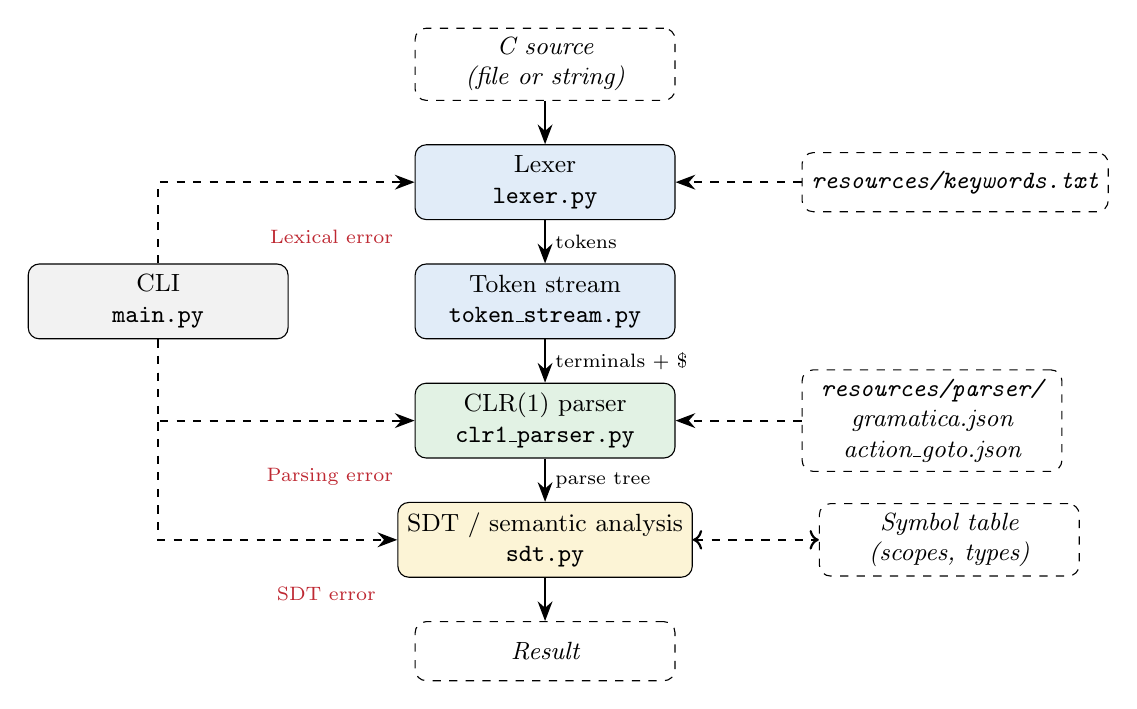
\begin{tikzpicture}[
  node distance=0.55cm,
  box/.style={draw, rounded corners, minimum width=3.3cm, minimum height=0.95cm, align=center, font=\small},
  data/.style={draw, dashed, rounded corners, minimum width=3.3cm, minimum height=0.75cm, align=center, font=\small\itshape},
  arr/.style={-{Stealth[length=2.5mm]}, thick}]
  \node[data] (src) {C source\\(file or string)};
  \node[box, fill=boxblue, below=of src] (lex) {Lexer\\\texttt{lexer.py}};
  \node[box, fill=boxblue, below=of lex] (ts) {Token stream\\\texttt{token\_stream.py}};
  \node[box, fill=boxgreen, below=of ts] (par) {CLR(1) parser\\\texttt{clr1\_parser.py}};
  \node[box, fill=boxyellow, below=of par] (sdt) {SDT / semantic analysis\\\texttt{sdt.py}};
  \node[data, below=of sdt] (out) {Result};

  \node[data, right=1.6cm of lex] (kw) {\texttt{resources/keywords.txt}};
  \node[data, right=1.6cm of par] (tab) {\texttt{resources/parser/}\\gramatica.json\\action\_goto.json};
  \node[data, right=1.6cm of sdt] (sym) {Symbol table\\(scopes, types)};
  \node[box, left=1.6cm of ts, fill=gray!10] (main) {CLI\\\texttt{main.py}};

  \draw[arr] (src) -- (lex);
  \draw[arr] (lex) -- node[right,font=\scriptsize]{tokens} (ts);
  \draw[arr] (ts) -- node[right,font=\scriptsize]{terminals + \$} (par);
  \draw[arr] (par) -- node[right,font=\scriptsize]{parse tree} (sdt);
  \draw[arr] (sdt) -- (out);
  \draw[arr,dashed] (kw) -- (lex);
  \draw[arr,dashed] (tab) -- (par);
  \draw[arr,<->,dashed] (sdt) -- (sym);
  \draw[arr,dashed] (main) |- (lex);
  \draw[arr,dashed] (main) |- (par);
  \draw[arr,dashed] (main) |- (sdt);

  \node[font=\scriptsize, text=errred, left=0.15cm of lex.south west, anchor=north east] {Lexical error};
  \node[font=\scriptsize, text=errred, left=0.15cm of par.south west, anchor=north east] {Parsing error};
  \node[font=\scriptsize, text=errred, left=0.15cm of sdt.south west, anchor=north east] {SDT error};
\end{tikzpicture}
\caption{Architecture of the project. Each phase stops the pipeline when it
finds an error, so a later phase only runs on a valid input.}
\label{fig:arch}
\end{figure}

\par\noindent\begin{minipage}{\linewidth}
\begin{lstlisting}
07/
|-- resources/
|   |-- keywords.txt          # print, int, float, char, return, if, else, while
|   `-- parser/               # gramatica.json + action_goto.json (Model Designer)
|-- src/main/
|   |-- lexer.py              # lexer of the previous project (+ float/char/while)
|   |-- token_stream.py       # bridge lexer -> parser: tokens to terminals + $
|   |-- clr1_parser.py        # CLR(1) engine: shift/reduce/goto/accept, tree
|   |-- sdt.py                # SDT: symbol table, scopes and types
|   `-- main.py               # command line interface
|-- examples/
`-- tests/                    # pytest + tests/cases (42 programs)
\end{lstlisting}
\end{minipage}\par


The grammar and the parsing table are \emph{data}: the parser reads them from
JSON files instead of hard-coding them. This keeps the theoretical model of
the Model Designer and the implementation consistent: the same productions
0--50 and states 0--160 appear in the documents, in the JSON files and in the
traces printed by the program.

% =====================================================================
\section{Lexical analyzer integration}
% =====================================================================

As the statement requires, the input of the parser is the output of a lexical
analyzer. The parser never reads characters: \texttt{token\_stream.py} runs
the lexer of the first project and translates each token into a
\emph{terminal} of the grammar. For this project the lexer was extended with
the keywords \texttt{float}, \texttt{char} and \texttt{while}, character
literals (\texttt{\textquotesingle{}c\textquotesingle{}}) and the operators \texttt{\%} and \texttt{!}.

The translation rules are shown in Table~\ref{tab:map}. Keywords, operators
and punctuation use their own lexeme as terminal; identifiers become
\tok{ID}; constants and literals become \tok{INT}, \tok{FLOAT}, \tok{CHAR} or
\tok{STRING}. The identifier \texttt{main} is still an identifier for the
lexer (in C it is not a reserved word), but it is mapped to the terminal
\tok{main} because the grammar expects \texttt{int main ( ) Block}. Finally,
the end-of-input marker \tok{\$} is appended exactly once.

\begin{table}[!htbp]
\centering
\caption{Translation from lexer tokens to grammar terminals.}
\label{tab:map}
\begin{tabular}{@{}lll@{}}
\toprule
\textbf{Lexer token} & \textbf{Example} & \textbf{Terminal} \\
\midrule
\tok{KEYWORD}     & \texttt{int}, \texttt{while}   & the lexeme: \tok{int}, \tok{while} \\
\tok{IDENTIFIER}  & \texttt{main}                  & \tok{main} \\
\tok{IDENTIFIER}  & \texttt{x}, \texttt{suma}      & \tok{ID} \\
\tok{CONSTANT}    & \texttt{10} / \texttt{3.5}     & \tok{INT} / \tok{FLOAT} \\
\tok{LITERAL}     & \texttt{\textquotesingle{}a\textquotesingle{}} / \texttt{"hola"} & \tok{CHAR} / \tok{STRING} \\
\tok{OPERATOR}    & \texttt{=}, \texttt{<=}        & the lexeme: \tok{=}, \tok{<=} \\
\tok{PUNCTUATION} & \texttt{;}, \texttt{\{}        & the lexeme: \tok{;}, \tok{\{} \\
end of input      & --                             & \tok{\$} \\
\bottomrule
\end{tabular}
\end{table}

Every terminal keeps a reference to its original token (lexeme, line and
column). That is what allows the parser and the SDT to report \emph{the line}
of an error. If the lexer reports any error, \texttt{token\_stream.py} raises
\texttt{LexicalError} and the parser is never called: an invalid token stream
is never treated as valid parser input. Figure~\ref{fig:flow} shows the flow
for one declaration, and Figures~\ref{fig:tokens} and \ref{fig:terminals}
show the real output of both stages for the same program.

\begin{figure}[!htbp]
\centering
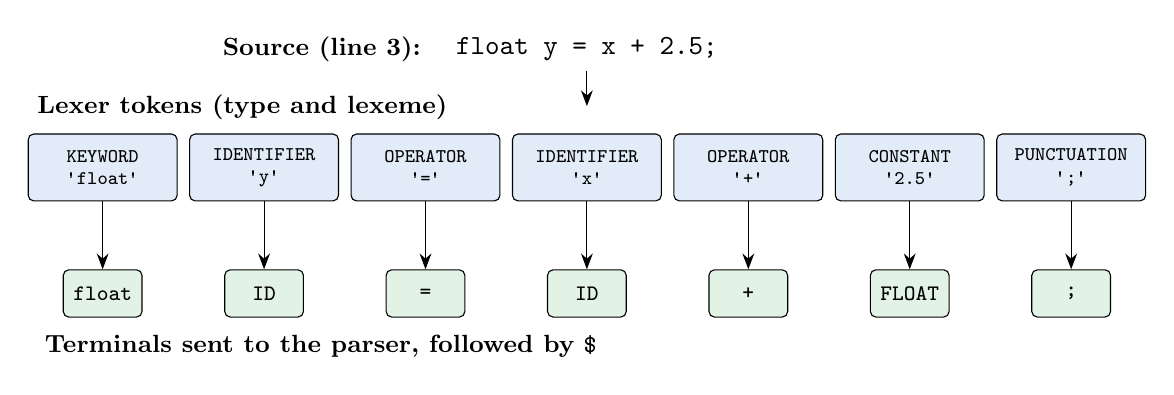
\begin{tikzpicture}[
  t/.style={draw, rounded corners=2pt, font=\ttfamily\scriptsize, text width=1.75cm, align=center, minimum height=0.85cm, inner sep=2pt, fill=boxblue},
  s/.style={draw, rounded corners=2pt, font=\ttfamily\footnotesize, minimum width=1.0cm, minimum height=0.6cm, inner sep=2pt, fill=boxgreen},
  arr/.style={-{Stealth[length=2mm]}}]
  \node[font=\ttfamily] (c) at (0,0.2) {float y = x + 2.5;};
  \node[left=0.2cm of c, font=\small\bfseries] {Source (line 3):};
  \foreach \i/\ty/\lx in {1/KEYWORD/float, 2/IDENTIFIER/y, 3/OPERATOR/=, 4/IDENTIFIER/x, 5/OPERATOR/+, 6/CONSTANT/2.5, 7/PUNCTUATION/;}
     \node[t] (k\i) at ({(\i-4)*2.05},-1.3) {\ty\\\textquotesingle\lx\textquotesingle};
  \foreach \i/\lab in {1/float, 2/ID, 3/=, 4/ID, 5/+, 6/FLOAT, 7/;}
     \node[s] (p\i) at ({(\i-4)*2.05},-2.9) {\lab};
  \foreach \i in {1,...,7} \draw[arr] (k\i) -- (p\i);
  \draw[arr] (c.south) -- ++(0,-0.45);
  \node[font=\small\bfseries, anchor=south west] at ($(k1.north west)+(0,0.05)$) {Lexer tokens (type and lexeme)};
  \node[font=\small\bfseries, anchor=north west] at ($(p1.south west)+(-0.35,-0.1)$) {Terminals sent to the parser, followed by \texttt{\$}};
\end{tikzpicture}
\caption{Lexer-to-parser token flow: each token keeps its lexeme, line and
column, but the parser only looks at the terminal symbol.}
\label{fig:flow}
\end{figure}

\begin{figure}[!htbp]
\centering
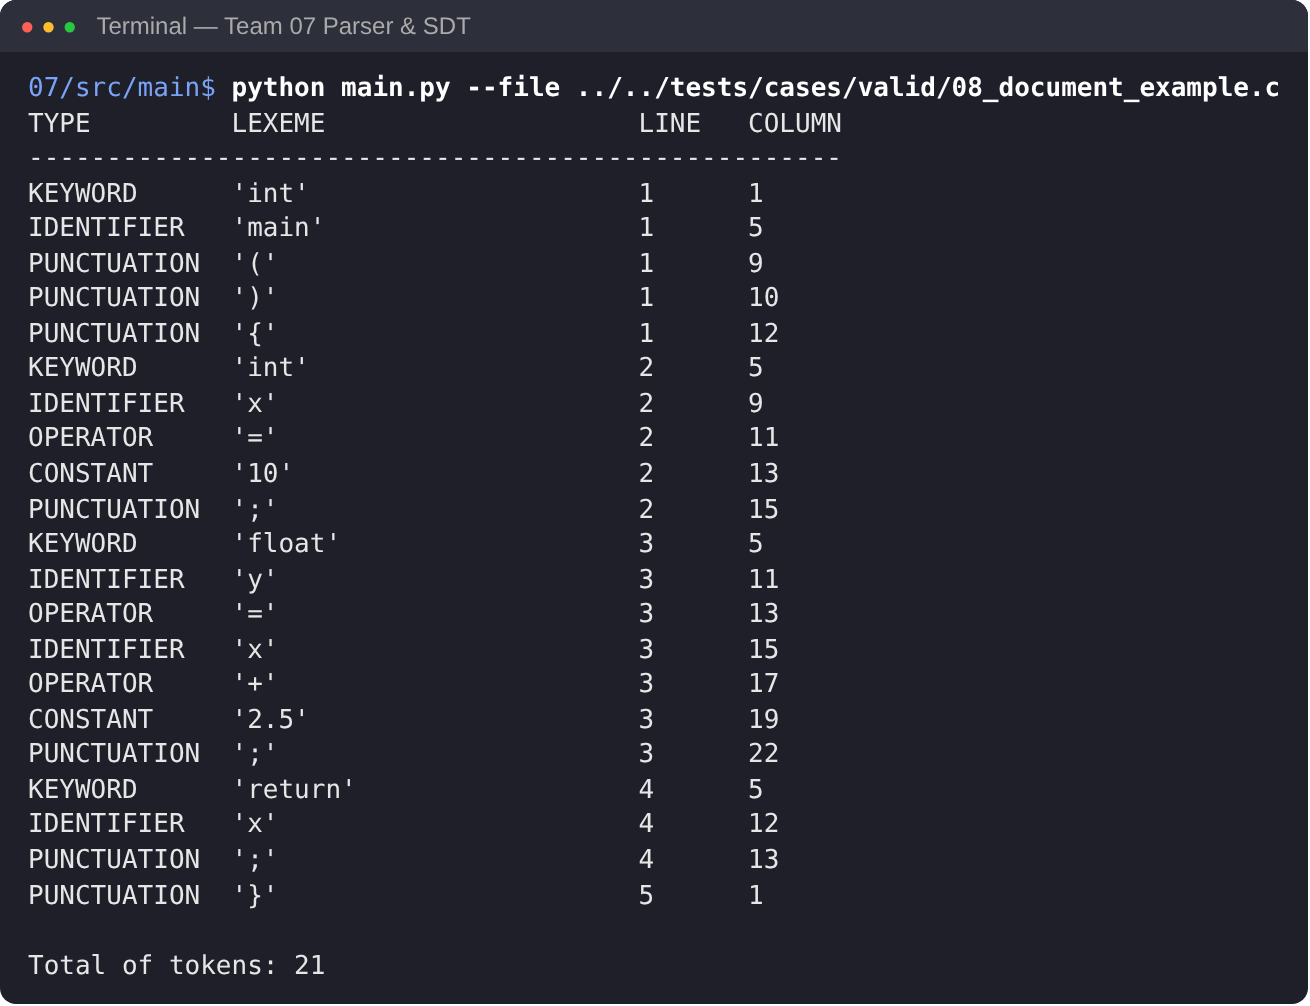
\includegraphics[width=0.66\linewidth]{shot_tokens.png}
\caption{Tokens produced by the lexer for \texttt{valid/08\_document\_example.c}.}
\label{fig:tokens}
\end{figure}

\begin{figure}[!htbp]
\centering
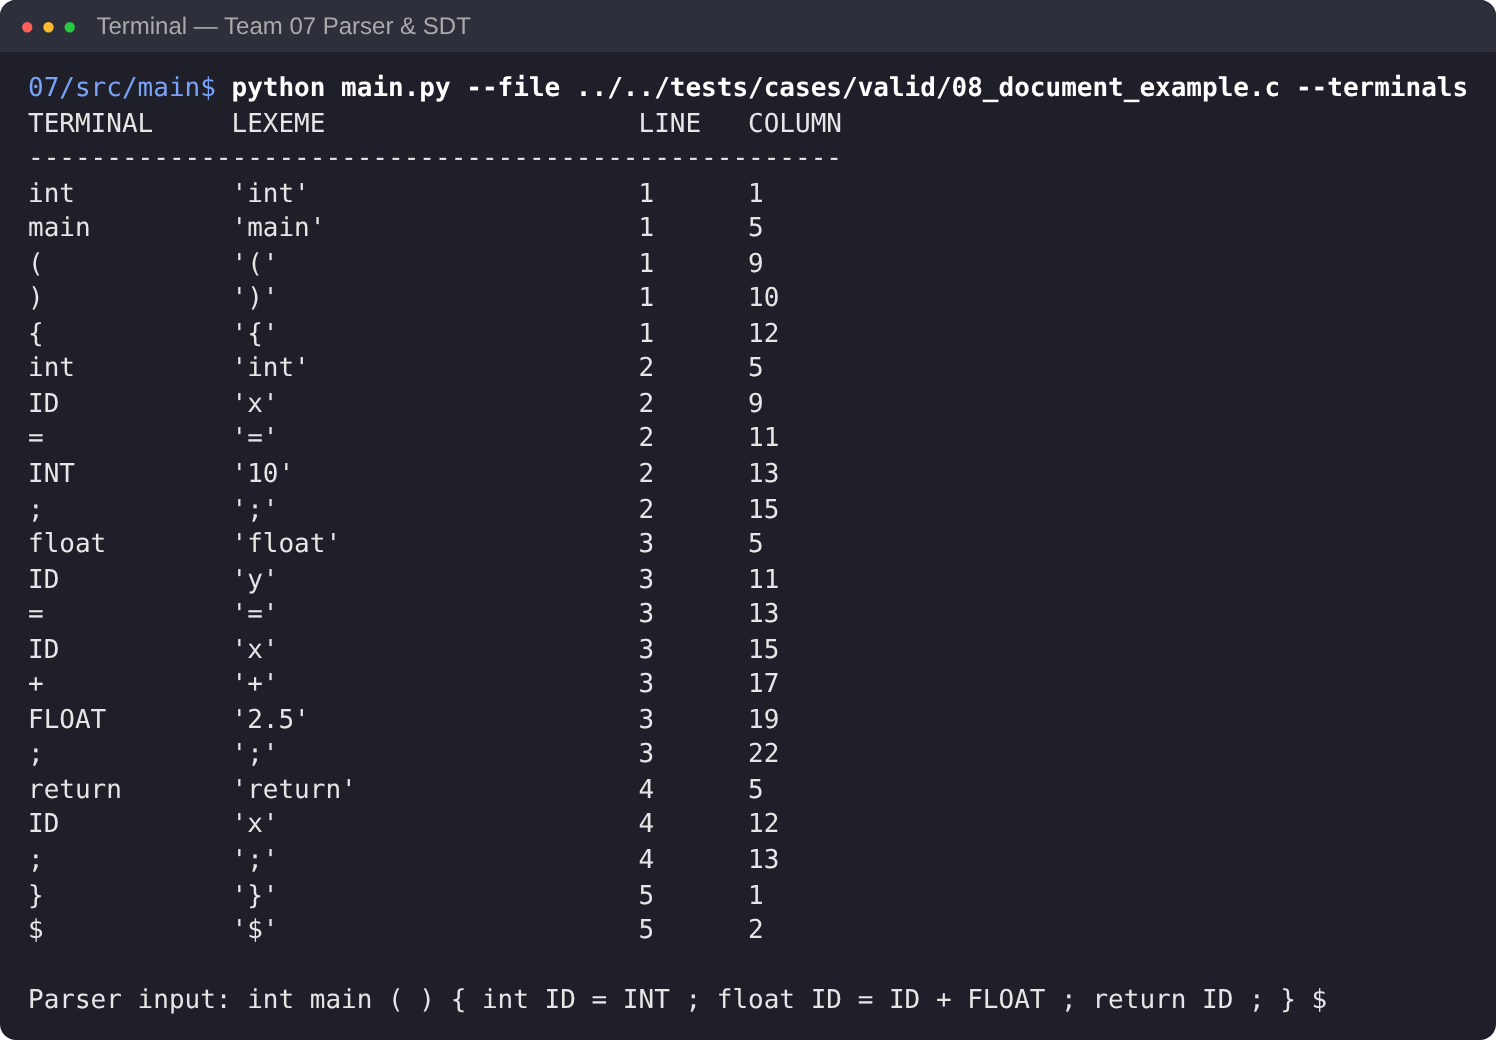
\includegraphics[width=0.72\linewidth]{shot_terminals.png}
\caption{The same program translated into grammar terminals; the last line
is the exact input that the CLR(1) parser receives.}
\label{fig:terminals}
\end{figure}

% =====================================================================
\FloatBarrier
\section{CLR(1) theoretical background}
% =====================================================================

\subsection{Bottom-up parsing}

A bottom-up parser builds the parse tree from the leaves (the tokens) up to
the root (the start symbol). It is a \emph{shift-reduce} parser: it keeps a
stack, \textbf{shifts} input symbols onto it and, when the top of the stack
matches the right-hand side of a production (a \emph{handle}),
\textbf{reduces} it to the left-hand side. Read in reverse, the sequence of
reductions is a rightmost derivation of the input \cite{aho2006}.

The LR family of parsers (\emph{L}eft-to-right scan, \emph{R}ightmost
derivation in reverse) decides when to shift and when to reduce by means of a
deterministic finite automaton whose states are sets of \emph{items}. The
decisions are stored in two tables:
\begin{itemize}
  \item \textbf{ACTION}[$i$, $a$], for a state $i$ and a terminal $a$:
        \emph{shift} $j$, \emph{reduce} by production $k$, \emph{accept}, or
        \emph{error} (empty cell).
  \item \textbf{GOTO}[$i$, $A$], for a state $i$ and a nonterminal $A$: the
        state reached after reducing to $A$.
\end{itemize}

\subsection{LR(1) items}

An LR(0) item is a production with a dot in its right-hand side, such as
$A\to\alpha\cdot\beta$: $\alpha$ has already been recognized and $\beta$ is
expected next. An \textbf{LR(1) item} adds a \emph{lookahead} terminal:
\[
[A\to\alpha\cdot\beta,\ a]
\]
which means ``we are recognizing $A\to\alpha\beta$, and after $A$ the next
input symbol must be $a$''. When the dot reaches the end, $[A\to\alpha\cdot,a]$
authorizes the reduction by $A\to\alpha$ \emph{only} when the next input
symbol is $a$.

\subsection{Why CLR(1)}

The methods seen in class differ in \emph{where} they place the reductions:

\begin{itemize}
  \item \textbf{LR(0)} reduces in every column of the row, regardless of the
        next symbol. Almost any realistic grammar has conflicts.
  \item \textbf{SLR(1)} reduces $A\to\alpha$ on every terminal of
        $\text{FOLLOW}(A)$. FOLLOW is global for the whole grammar, so it can
        authorize reductions in contexts where they are not valid, which
        produces shift/reduce and reduce/reduce conflicts.
  \item \textbf{CLR(1)} (canonical LR(1)) reduces only on the lookahead of the
        specific item, computed in its context. It is the most powerful of these
        methods: every SLR(1) and LALR(1) grammar is CLR(1). LR(k) parsing
        was introduced by Knuth \cite{knuth1965}.
  \item \textbf{LALR(1)} merges CLR(1) states with the same LR(0) core; it has
        fewer states but can introduce reduce/reduce conflicts.
\end{itemize}

The team chose \textbf{CLR(1)} because the goal was to cover a broad and
realistic subset of C: nested statements, the \emph{dangling else}, and an
expression grammar with six precedence levels. The extra precision of the
lookaheads means that the grammar can be written naturally (left recursion,
$\varepsilon$-productions) without conflicts. A concrete example appears in
the collection: states $I_9$ and $I_{122}$ have the same core
\texttt{Simple -> ; .}, but only $I_{122}$ has \tok{else} as a lookahead. In
CLR(1) they are kept as different states, so the reduction by p24 is
authorized before \tok{else} only where it is valid. The price of CLR(1) is a
larger number of states (161), which is not a problem because the table is
computed once and stored as data.

\subsection{CLOSURE and GOTO}
\label{sec:closure}

The canonical collection is built with two operations \cite{aho2006}:

\textbf{CLOSURE($I$).} If $[A\to\alpha\cdot B\beta,\ a]$ is in $I$ and
$B\to\gamma$ is a production, add $[B\to\cdot\gamma,\ b]$ for every terminal
$b\in\text{FIRST}(\beta a)$. Repeat until no new item can be added. The
lookahead $b$ is computed from what follows $B$ \emph{in this item}
($\beta$), and only if $\beta$ can derive $\varepsilon$ does the original
lookahead $a$ propagate.

\textbf{GOTO($I$, $X$).} Move the dot over the symbol $X$ in every item of
$I$ that has $X$ right after the dot, and apply CLOSURE to the result.

The collection starts with $I_0=\text{CLOSURE}(\{[\texttt{Start}\to\cdot\texttt{Program},\ \$]\})$
and applies GOTO with every grammar symbol to every state until no new set of
items appears.

\textbf{Example in the team's collection (state $I_{28}$).} After reading
\texttt{int x} inside a block, the parser is in $I_{28}$, which contains
\[
[\texttt{Decl}\to\texttt{Type ID}\cdot\texttt{Init ;},\ a].
\]
The symbol after the dot is the nonterminal \texttt{Init} and the rest of the
item is $\beta=\texttt{;}$, so $\text{FIRST}(\beta a)=\text{FIRST}(\texttt{;}\,a)=\{\texttt{;}\}$.
CLOSURE therefore adds both productions of \texttt{Init} with lookahead
\texttt{;}:
\[
[\texttt{Init}\to\cdot\ \texttt{= Expr},\ \texttt{;}]\qquad
[\texttt{Init}\to\cdot,\ \texttt{;}]
\]
The first item lets the parser shift \tok{=} (GOTO($I_{28}$,\,=)\,=\,$I_{49}$).
The second is already complete, so it authorizes the reduction
\texttt{Init -> $\varepsilon$} (p12) \emph{only} before \tok{;}. That is
exactly what happens in \texttt{int x;}. After the reduction,
GOTO($I_{28}$,\,Init)\,=\,$I_{50}$ contains
$[\texttt{Decl}\to\texttt{Type ID Init}\cdot\texttt{;},\ a]$.

\subsection{Construction of the ACTION/GOTO table}

For every state $I_i$ of the collection:
\begin{enumerate}
  \item If GOTO($I_i$, $t$) $=I_j$ and $t$ is a terminal, ACTION[$i$, $t$] $=$ shift $j$.
  \item If $[A\to\alpha\cdot,\ a]\in I_i$ and $A\ne\texttt{Start}$,
        ACTION[$i$, $a$] $=$ reduce by $A\to\alpha$ (only in column $a$).
  \item If $[\texttt{Start}\to\texttt{Program}\cdot,\ \$]\in I_i$,
        ACTION[$i$, \$] $=$ accept.
  \item If GOTO($I_i$, $A$) $=I_j$ and $A$ is a nonterminal, GOTO[$i$, $A$] $=j$.
\end{enumerate}
A cell that receives two different actions is a \emph{conflict}; the grammar is
CLR(1) if and only if no cell has a conflict.

\subsection{The LR parsing algorithm}

With the table, the driver is the same for every LR method:

\par\noindent\begin{minipage}{\linewidth}
\begin{lstlisting}
push state 0;  a = first terminal
loop:
    s = state on top of the stack
    case ACTION[s, a] of
      shift j:   push j;  a = next terminal
      reduce k:  (A -> beta) = production k
                 pop |beta| states;  t = new top
                 push GOTO[t, A];  build node A with the popped children
      accept:    return the tree (Parsing Success!)
      empty:     syntax error in the line of a
\end{lstlisting}
\end{minipage}\par


A reduce does not consume input, and a reduce by an $\varepsilon$-production
pops nothing; it only pushes the GOTO state.

% =====================================================================
\FloatBarrier
\section{Grammar definition}
% =====================================================================

A context-free grammar is a 4-tuple $G=(N,T,P,S)$ of nonterminals,
terminals, productions and start symbol \cite{hopcroft2007}. The grammar of
this project was designed by the Model Designer on top of the
tokens of the lexer \cite{md}.

\textbf{Terminals} ($|T|=31$, plus \tok{\$} as the 32nd ACTION column):
\begin{center}
\texttt{! != \% ( ) * + - / ; < <= = == > >= CHAR FLOAT ID INT STRING}\\
\texttt{char else float if int main return while \{ \}}
\end{center}

\textbf{Nonterminals} ($|N|=18$): \texttt{Program, Block, Items, Item, Decl,
Type, Init, Stmt, Matched, Unmatched, Simple, Expr, Equality, Relation, Add,
Mul, Unary, Primary}.

\textbf{Start symbol:} \texttt{Program}.

\textbf{Productions:} the 51 productions are listed in
Table~\ref{tab:prods}. Their numbers are the ones used by the parsing table,
the reductions of the trace and the SDT rules.

{\small
\setlength{\tabcolsep}{4pt}
\begin{longtable}{@{}l l l | l l l@{}}
\caption{Productions of the grammar (p0 is the augmentation).}\label{tab:prods}\\
\toprule
\textbf{\#} & \textbf{LHS} & \textbf{RHS} & \textbf{\#} & \textbf{LHS} & \textbf{RHS}\\
\midrule
\endfirsthead
\toprule
\textbf{\#} & \textbf{LHS} & \textbf{RHS} & \textbf{\#} & \textbf{LHS} & \textbf{RHS}\\
\midrule
\endhead
p0 & \texttt{Start} & \texttt{Program} & p26 & \texttt{Equality} & \texttt{Equality == Relation}\\
p1 & \texttt{Program} & \texttt{int main ( ) Block} & p27 & \texttt{Equality} & \texttt{Equality != Relation}\\
p2 & \texttt{Block} & \texttt{\{ Items \}} & p28 & \texttt{Equality} & \texttt{Relation}\\
p3 & \texttt{Items} & \texttt{Items Item} & p29 & \texttt{Relation} & \texttt{Relation \textless{} Add}\\
p4 & \texttt{Items} & \texttt{$\varepsilon$} & p30 & \texttt{Relation} & \texttt{Relation \textless{}= Add}\\
p5 & \texttt{Item} & \texttt{Decl} & p31 & \texttt{Relation} & \texttt{Relation \textgreater{} Add}\\
p6 & \texttt{Item} & \texttt{Stmt} & p32 & \texttt{Relation} & \texttt{Relation \textgreater{}= Add}\\
p7 & \texttt{Decl} & \texttt{Type ID Init ;} & p33 & \texttt{Relation} & \texttt{Add}\\
p8 & \texttt{Type} & \texttt{int} & p34 & \texttt{Add} & \texttt{Add + Mul}\\
p9 & \texttt{Type} & \texttt{float} & p35 & \texttt{Add} & \texttt{Add - Mul}\\
p10 & \texttt{Type} & \texttt{char} & p36 & \texttt{Add} & \texttt{Mul}\\
p11 & \texttt{Init} & \texttt{= Expr} & p37 & \texttt{Mul} & \texttt{Mul * Unary}\\
p12 & \texttt{Init} & \texttt{$\varepsilon$} & p38 & \texttt{Mul} & \texttt{Mul / Unary}\\
p13 & \texttt{Stmt} & \texttt{Matched} & p39 & \texttt{Mul} & \texttt{Mul \% Unary}\\
p14 & \texttt{Stmt} & \texttt{Unmatched} & p40 & \texttt{Mul} & \texttt{Unary}\\
p15 & \texttt{Matched} & \texttt{Simple} & p41 & \texttt{Unary} & \texttt{+ Unary}\\
p16 & \texttt{Matched} & \texttt{Block} & p42 & \texttt{Unary} & \texttt{- Unary}\\
p17 & \texttt{Matched} & \texttt{if ( Expr ) Matched else Matched} & p43 & \texttt{Unary} & \texttt{! Unary}\\
p18 & \texttt{Matched} & \texttt{while ( Expr ) Matched} & p44 & \texttt{Unary} & \texttt{Primary}\\
p19 & \texttt{Unmatched} & \texttt{if ( Expr ) Stmt} & p45 & \texttt{Primary} & \texttt{ID}\\
p20 & \texttt{Unmatched} & \texttt{if ( Expr ) Matched else Unmatched} & p46 & \texttt{Primary} & \texttt{INT}\\
p21 & \texttt{Unmatched} & \texttt{while ( Expr ) Unmatched} & p47 & \texttt{Primary} & \texttt{FLOAT}\\
p22 & \texttt{Simple} & \texttt{ID = Expr ;} & p48 & \texttt{Primary} & \texttt{CHAR}\\
p23 & \texttt{Simple} & \texttt{return Expr ;} & p49 & \texttt{Primary} & \texttt{STRING}\\
p24 & \texttt{Simple} & \texttt{;} & p50 & \texttt{Primary} & \texttt{( Expr )}\\
p25 & \texttt{Expr} & \texttt{Equality} &  & & \\
\bottomrule
\end{longtable}
}

\subsection{Design decisions of the grammar}

\begin{itemize}
  \item \textbf{Program and blocks.} \texttt{Program -> int main ( ) Block}
        and \texttt{Block -> \{ Items \}}. \texttt{Items} is a left-recursive
        list that can be empty (p3, p4). Left recursion is natural for LR
        parsers: the list is reduced as soon as each item ends, so the stack
        does not grow with the length of the program.
  \item \textbf{Declarations vs.\ assignments.} A declaration begins with
        \texttt{Type} (\texttt{Decl -> Type ID Init ;}), an assignment begins
        with \tok{ID} (\texttt{Simple -> ID = Expr ;}). The optional
        initializer is \texttt{Init -> = Expr | $\varepsilon$}.
  \item \textbf{Dangling else.} Statements are split into \texttt{Matched}
        (every \texttt{if} has its \texttt{else}) and \texttt{Unmatched}
        (some \texttt{if} is still open). Only a \texttt{Matched} statement
        can appear between \texttt{if (...)} and \texttt{else}, so every
        \texttt{else} is attached to the nearest open \texttt{if}. The
        ambiguity is removed by the grammar itself, not by giving priority to
        shift in the table.
  \item \textbf{Precedence and associativity.} One nonterminal per level, from
        lowest to highest: \texttt{Equality} (\texttt{== !=}),
        \texttt{Relation} (\texttt{< <= > >=}), \texttt{Add} (\texttt{+ -}),
        \texttt{Mul} (\texttt{* / \%}), \texttt{Unary} (prefix \texttt{+ - !})
        and \texttt{Primary}. Binary levels are left-recursive (left
        associative): \texttt{8 - 3 - 1} is \texttt{(8 - 3) - 1}; prefix
        operators are right-recursive. Thus \texttt{1 + 2 * 3} is
        \texttt{1 + (2 * 3)} because \texttt{Add} uses a whole \texttt{Mul}
        as its right operand.
  \item \textbf{Assignment is a statement.} The assignment is not part of
        \texttt{Expr}, which keeps \texttt{=} out of expressions.
\end{itemize}

\subsection{The professor's example}
\label{sec:prof}

The unit recognized by \texttt{Program} is a complete \texttt{main} function.
The declaration \texttt{int x = 10;} is generated by the grammar, but inside
a block: \texttt{Decl -> Type ID Init ;} with \texttt{Type -> int},
\texttt{Init -> = Expr} and the chain \texttt{Expr} $\Rightarrow^{*}$
\texttt{Primary -> INT}. On its own it is not a \texttt{Program}: in state
$I_0$ the only valid action is \emph{shift} \tok{int}, which leads to
$I_2$, where the parser requires \tok{main}. The terminal after \tok{int} is
\tok{ID}, so ACTION[2, ID] is empty and the result is
\bad{Parsing error in line 1}. Placed inside \texttt{main}, which is how it
appears in a real C program, the same declaration produces
\ok{Parsing Success!} and \ok{SDT Verified!} (Figure~\ref{fig:prof}).

\begin{figure}[!htbp]
\centering
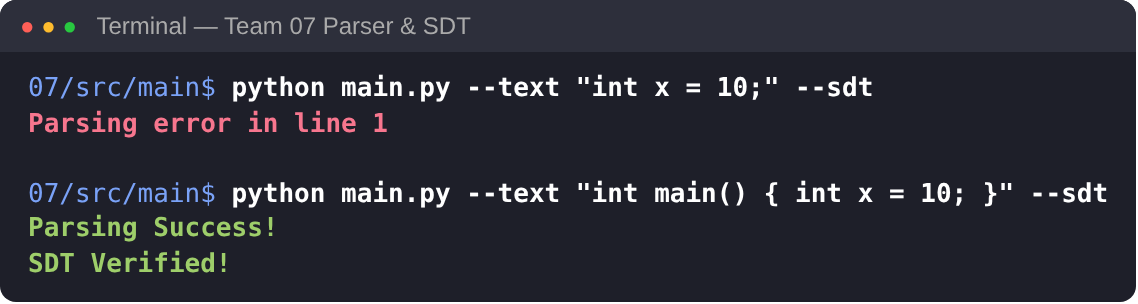
\includegraphics[width=0.66\linewidth]{shot_prof.png}
\caption{The professor's example alone and inside \texttt{int main()}.}
\label{fig:prof}
\end{figure}

% =====================================================================
\section{Augmented grammar}
% =====================================================================

To know exactly when the input has been completely recognized, the grammar is
\emph{augmented} with a new start symbol and the production
\[
\text{p0:}\quad \texttt{Start} \to \texttt{Program}
\]
The parser accepts when, with the item $[\texttt{Start}\to\texttt{Program}\cdot,\ \$]$
on top of the stack, it reads \tok{\$}. Without this production the parser
could not tell the reduction to \texttt{Program} at the end of the input from
any other reduction. p0 is never used as an ordinary reduction: its complete
item generates ACCEPT in ACTION[1, \$], and \texttt{Start} has no column in
the GOTO table, which therefore uses only the 18 original nonterminals.

The FIRST sets used by CLOSURE are listed in Table~\ref{tab:first}.

\begin{table}[!htbp]
\centering
\caption{FIRST sets of the nonterminals.}
\label{tab:first}
\small
\begin{tabularx}{\linewidth}{@{}p{5.3cm}X@{}}
\toprule
\textbf{Nonterminal(s)} & \textbf{FIRST} \\
\midrule
\texttt{Start, Program} & \texttt{int} \\
\texttt{Block} & \texttt{\{} \\
\texttt{Items} & \texttt{; ID char float if int return while \{} $\varepsilon$ \\
\texttt{Item} & \texttt{; ID char float if int return while \{} \\
\texttt{Decl, Type} & \texttt{char float int} \\
\texttt{Init} & \texttt{=} $\varepsilon$ \\
\texttt{Stmt, Matched} & \texttt{; ID if return while \{} \\
\texttt{Unmatched} & \texttt{if while} \\
\texttt{Simple} & \texttt{; ID return} \\
\texttt{Expr, Equality, Relation, Add, Mul, Unary} & \texttt{! ( + - CHAR FLOAT ID INT STRING} \\
\texttt{Primary} & \texttt{( CHAR FLOAT ID INT STRING} \\
\bottomrule
\end{tabularx}
\end{table}

% =====================================================================
\section{Canonical collection of LR(1) items}
% =====================================================================

Applying CLOSURE and GOTO (Section~\ref{sec:closure}) from
$I_0=\text{CLOSURE}(\{[\texttt{Start}\to\cdot\texttt{Program},\ \$]\})$
produces \textbf{161 distinct states} ($I_0$--$I_{160}$) and \textbf{730
transitions}. No two states are merged, even if they share the same LR(0)
core, because that is the definition of the canonical collection. The
complete collection is in the Model Designer document \cite{md} and in
\texttt{docs/model-designer/Datos/coleccion\_lr1.json}. Some representative
states are:

\par\noindent\begin{minipage}{\linewidth}
\begin{lstlisting}
I0 : [Start -> . Program , $]
     [Program -> . int main ( ) Block , $]
I1 : [Start -> Program . , $]                                   (accept)
I5 : [Program -> int main ( ) . Block , $]
     [Block -> . { Items } , $]
I7 : [Block -> { . Items } , $]
     [Items -> . Items Item , ; ID char float if int return while { }]
     [Items -> . , ; ID char float if int return while { }]
I17: [Decl -> Type . ID Init ; , ; ID char float if int return while { }]
I22: [Type -> int . , ID]
I28: [Decl -> Type ID . Init ; , ; ID char float if int return while { }]
     [Init -> . = Expr , ;]
     [Init -> . , ;]
I50: [Decl -> Type ID Init . ; , ; ID char float if int return while { }]
I87: [Decl -> Type ID Init ; . , ; ID char float if int return while { }]
\end{lstlisting}
\end{minipage}\par


In $I_7$ the lookaheads of \texttt{Items} are the FIRST of what can follow a
list inside a block: the start of another \texttt{Item} or the closing brace
\tok{\}}. In $I_{22}$ the only lookahead of \texttt{Type -> int .} is \tok{ID},
because after a type the grammar always expects the name of the variable.
Figure~\ref{fig:dfa} shows the path of the automaton that recognizes
\texttt{int main() \{ int x; \}} and \texttt{int main() \{ int x = ... \}}.

\begin{figure}[!htbp]
\centering
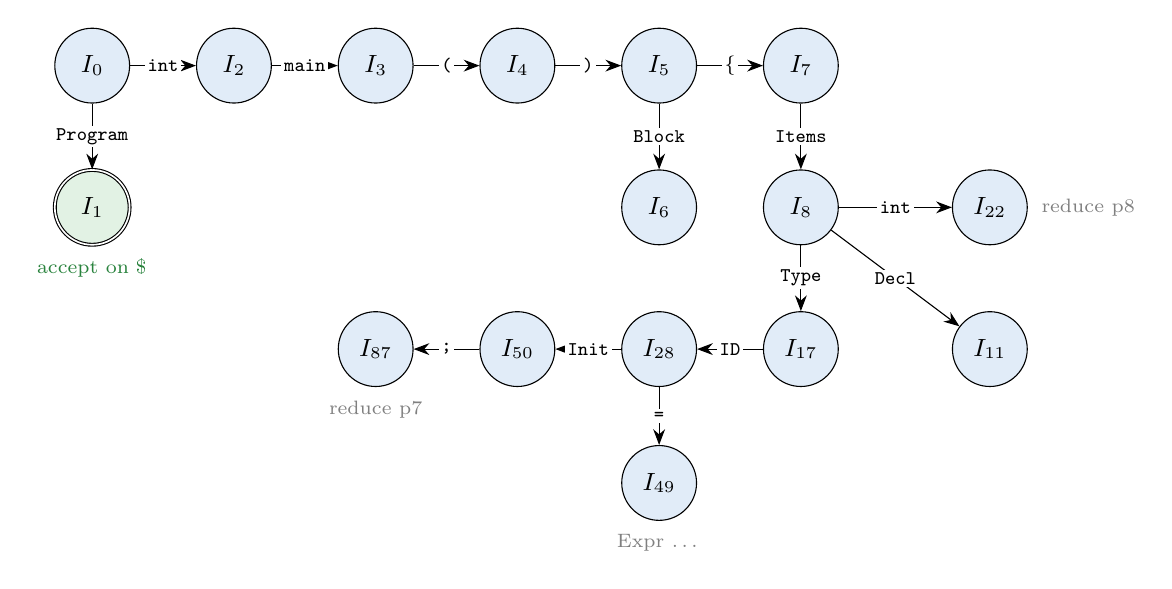
\begin{tikzpicture}[
  st/.style={draw, circle, minimum size=0.95cm, font=\small, fill=boxblue},
  acc/.style={st, double, fill=boxgreen},
  arr/.style={-{Stealth[length=2mm]}},
  lab/.style={font=\scriptsize\ttfamily, fill=white, inner sep=1pt}]
  \node[st] (0) at (0,0) {$I_0$};
  \node[acc] (1) at (0,-1.8) {$I_1$};
  \node[st] (2) at (1.8,0) {$I_2$};
  \node[st] (3) at (3.6,0) {$I_3$};
  \node[st] (4) at (5.4,0) {$I_4$};
  \node[st] (5) at (7.2,0) {$I_5$};
  \node[st] (6) at (7.2,-1.8) {$I_6$};
  \node[st] (7) at (9.0,0) {$I_7$};
  \node[st] (8) at (9.0,-1.8) {$I_8$};
  \node[st] (22) at (11.4,-1.8) {$I_{22}$};
  \node[st] (17) at (9.0,-3.6) {$I_{17}$};
  \node[st] (28) at (7.2,-3.6) {$I_{28}$};
  \node[st] (50) at (5.4,-3.6) {$I_{50}$};
  \node[st] (87) at (3.6,-3.6) {$I_{87}$};
  \node[st] (49) at (7.2,-5.3) {$I_{49}$};
  \node[st] (11) at (11.4,-3.6) {$I_{11}$};
  \draw[arr] (0) -- node[lab]{Program} (1);
  \draw[arr] (0) -- node[lab]{int} (2);
  \draw[arr] (2) -- node[lab]{main} (3);
  \draw[arr] (3) -- node[lab]{(} (4);
  \draw[arr] (4) -- node[lab]{)} (5);
  \draw[arr] (5) -- node[lab]{Block} (6);
  \draw[arr] (5) -- node[lab]{\{} (7);
  \draw[arr] (7) -- node[lab]{Items} (8);
  \draw[arr] (8) -- node[lab]{int} (22);
  \draw[arr] (8) -- node[lab]{Type} (17);
  \draw[arr] (8) -- node[lab]{Decl} (11);
  \draw[arr] (17) -- node[lab]{ID} (28);
  \draw[arr] (28) -- node[lab]{Init} (50);
  \draw[arr] (28) -- node[lab]{=} (49);
  \draw[arr] (50) -- node[lab]{;} (87);
  \node[font=\scriptsize, text=gray, below=0.05cm of 49] {Expr \dots};
  \node[font=\scriptsize, text=okgreen, below=0.05cm of 1] {accept on \$};
  \node[font=\scriptsize, text=gray, below=0.05cm of 87] {reduce p7};
  \node[font=\scriptsize, text=gray, right=0.05cm of 22] {reduce p8};
\end{tikzpicture}
\caption{Fragment of the CLR(1) automaton (states and transitions taken from
the team's collection).}
\label{fig:dfa}
\end{figure}

% =====================================================================
\section{ACTION/GOTO parsing table}
% =====================================================================

Applying the construction rules to the 161 states gives \textbf{509 shift
actions, 795 reduce actions, 1 accept and 221 GOTO entries}, with
\textbf{zero shift/reduce and zero reduce/reduce conflicts}. This proves that
the grammar is CLR(1). The parser double-checks this property when it loads
the table: if a cell contains more than one action, the table is rejected.
ACTION has 32 columns (31 terminals and \tok{\$}); GOTO has 18 columns.

Table~\ref{tab:action} shows the rows used by the examples of this report.
Each entry \texttt{action: terminals} means that the action applies to every
listed column; any column not listed is an error.

{\small
\setlength{\tabcolsep}{4pt}
\begin{longtable}{@{}r p{9.6cm} p{4.6cm}@{}}
\caption{Excerpt of the ACTION/GOTO table (complete table in \cite{md}).}\label{tab:action}\\
\toprule
\textbf{State} & \textbf{ACTION} & \textbf{GOTO}\\
\midrule
\endfirsthead
\toprule
\textbf{State} & \textbf{ACTION} & \textbf{GOTO}\\
\midrule
\endhead
0 & \texttt{\textbf{s2}: int} & \texttt{Program$\to$1}\\
1 & \texttt{\textbf{acc}: \$} & \texttt{--}\\
2 & \texttt{\textbf{s3}: main} & \texttt{--}\\
5 & \texttt{\textbf{s7}: \{} & \texttt{Block$\to$6}\\
6 & \texttt{\textbf{r1}: \$} & \texttt{--}\\
7 & \texttt{\textbf{r4}: ; ID char float if int return while \{ \}} & \texttt{Items$\to$8}\\
8 & \texttt{\textbf{s9}: ; \,\textbar\, \textbf{s12}: ID \,\textbar\, \textbf{s19}: char \,\textbar\, \textbf{s20}: float \,\textbar\, \textbf{s21}: if \,\textbar\, \textbf{s22}: int \,\textbar\, \textbf{s23}: return \,\textbar\, \textbf{s24}: while \,\textbar\, \textbf{s25}: \{ \,\textbar\, \textbf{s26}: \}} & \texttt{Block$\to$10, Decl$\to$11, Item$\to$13, Matched$\to$14, Simple$\to$15, Stmt$\to$16, Type$\to$17, Unmatched$\to$18}\\
17 & \texttt{\textbf{s28}: ID} & \texttt{--}\\
22 & \texttt{\textbf{r8}: ID} & \texttt{--}\\
28 & \texttt{\textbf{r12}: ; \,\textbar\, \textbf{s49}: =} & \texttt{Init$\to$50}\\
49 & \texttt{\textbf{s30}: ! \,\textbar\, \textbf{s31}: ( \,\textbar\, \textbf{s32}: + \,\textbar\, \textbf{s33}: - \,\textbar\, \textbf{s35}: CHAR \,\textbar\, \textbf{s38}: FLOAT \,\textbar\, \textbf{s39}: ID \,\textbar\, \textbf{s40}: INT \,\textbar\, \textbf{s44}: STRING} & \texttt{Add$\to$34, Equality$\to$36, Expr$\to$86, Mul$\to$41, Primary$\to$42, Relation$\to$43, Unary$\to$45}\\
50 & \texttt{\textbf{s87}: ;} & \texttt{--}\\
87 & \texttt{\textbf{r7}: ; ID char float if int return while \{ \}} & \texttt{--}\\
\bottomrule
\end{longtable}
}

How to read some cells:
\begin{itemize}
  \item ACTION[0, int] $=$ s2: the only way to start a program is the keyword
        \tok{int}. Any other first token is a syntax error in line 1.
  \item ACTION[7, $t$] $=$ r4 for the ten terminals that can start an item
        or close the block: the empty list \texttt{Items -> $\varepsilon$} is
        reduced without consuming the token.
  \item ACTION[28, ;] $=$ r12 and ACTION[28, =] $=$ s49: after
        \texttt{Type ID}, a \tok{;} means ``no initializer'' and \tok{=}
        starts one. Any other token (for example \tok{ID} in
        \texttt{int x y;}) is an error.
  \item ACTION[1, \$] $=$ acc: the whole input is a \texttt{Program}.
\end{itemize}

% =====================================================================
\section{Parser implementation}
% =====================================================================

The parser is in \texttt{clr1\_parser.py}. It does not compute the collection
at run time: \texttt{ParsingTable} loads \texttt{gramatica.json} (productions
\texttt{\{id, lhs, rhs\}}) and \texttt{action\_goto.json} (\texttt{["s", n]},
\texttt{["r", p]} or \texttt{["acc", 0]}), checks that no cell has two
actions, and builds two dictionaries indexed by (state, symbol).

\texttt{Parser.parse} is the LR algorithm of the previous section. It keeps
two parallel stacks: one of \emph{states} and one of \emph{tree nodes}.

\begin{itemize}
  \item \textbf{Shift $j$}: push $j$ and a leaf node with the terminal (it
        keeps lexeme, line and column), and advance the input.
  \item \textbf{Reduce $k$} ($A\to\beta$): look at the state exposed under
        the top $|\beta|$ states, consult GOTO for $A$, pop $|\beta|$ states
        and nodes, and push the GOTO state and a new node $A$ whose children
        are the popped nodes, in order. If $\beta=\varepsilon$, nothing is
        popped and the node has no children.
  \item \textbf{Accept}: return the root of the tree and print
        \ok{Parsing Success!}.
  \item \textbf{Empty cell}: raise \texttt{ParseError} with the line of the
        error and the list of terminals that were expected in that state.
\end{itemize}

With the option \texttt{-{}-trace} the parser records the stack, the
lookahead and the action of every step. Figure~\ref{fig:trace} shows the
complete execution for \texttt{int main() \{ int x; \}}. It matches the
theory step by step: the empty list (r4) and the empty initializer (r12) are
reduced without consuming the token; \texttt{Type -> int} is reduced as soon
as \tok{ID} appears (the only lookahead of $I_{22}$); the reduction by p7
pops four states (\texttt{Type ID Init ;}); and the input is accepted with
the stack \texttt{0 1} and the token \tok{\$}.

\begin{figure}[!htbp]
\centering
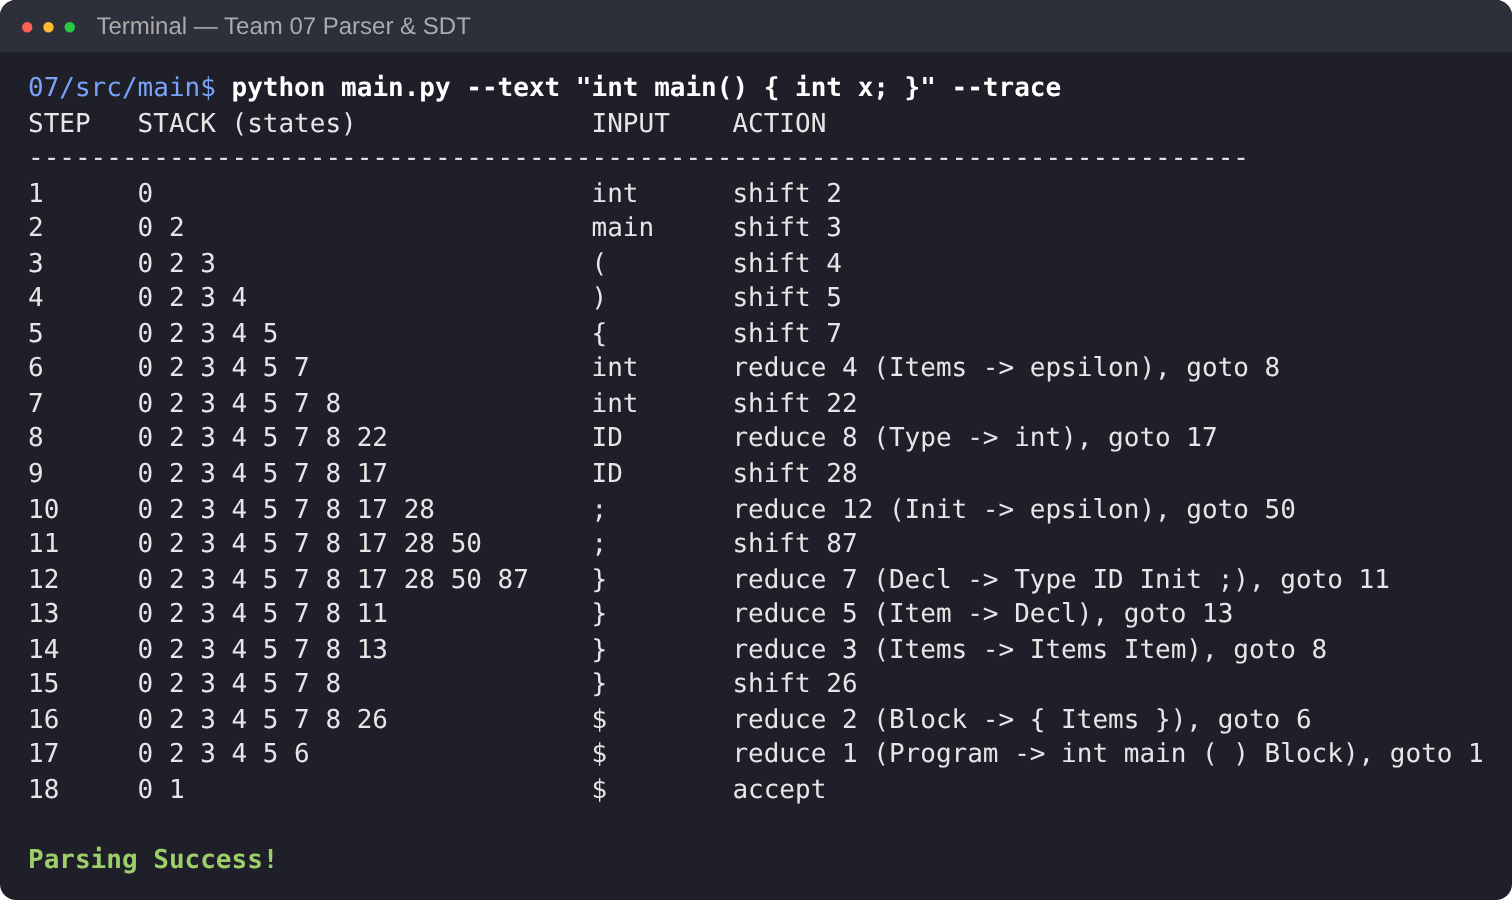
\includegraphics[width=0.95\linewidth]{shot_trace.png}
\caption{Parser execution: complete shift/reduce trace.}
\label{fig:trace}
\end{figure}

\subsection{Line of a syntax error}

An LR parser detects an error at the first token that cannot continue a valid
prefix. For most errors, that token is where the problem is. The exception is
a missing \tok{;} at the end of a line: the parser only notices it when it
reads the first token of the \emph{next} line. To report the line the
programmer expects, when the unexpected token starts a new line the parser
simulates inserting a \tok{;} before it (without changing the real stacks).
If the \tok{;} is accepted and the unexpected token can follow it, the
missing \tok{;} was the cause and the error is reported in the line of the
previous token; otherwise it is reported in the line of the unexpected token.

% =====================================================================
\section{Parse tree construction}
% =====================================================================

The tree is built bottom-up during the reductions, so it is a direct record of
the derivation: every internal node is a nonterminal together with the
production used to reduce it, and every leaf is a token. The root is
\texttt{Program}. Intermediate productions (\texttt{Expr -> Equality},
\texttt{Equality -> Relation}, \dots) are \emph{not} removed: each one is a
node, so the SDT rule of every production can be applied to its own node.
Figure~\ref{fig:forest} shows the subtree of the declaration
\texttt{int x = 10;}; Figure~\ref{fig:tree} shows the tree printed by the
program for a complete example.

\begin{figure}[!htbp]
\centering
\begin{forest}
  for tree={font=\small\ttfamily, draw, rounded corners=2pt, inner sep=2pt,
            fill=boxyellow, l sep=8pt, s sep=6pt, edge={-}},
  where n children=0{fill=boxblue}{}
  [Decl {(p7)}
    [Type {(p8)} [int]]
    [ID {'x'}]
    [Init {(p11)}
      [=]
      [Expr {(p25)} [Equality {(p28)} [Relation {(p33)} [Add {(p36)} [Mul {(p40)} [Unary {(p44)} [Primary {(p46)} [INT {'10'}]]]]]]]]
    ]
    [;]
  ]
\end{forest}
\caption{Parse subtree of \texttt{int x = 10;} (yellow: nonterminals with
their production; blue: leaves/tokens).}
\label{fig:forest}
\end{figure}

\begin{figure}[!htbp]
\centering
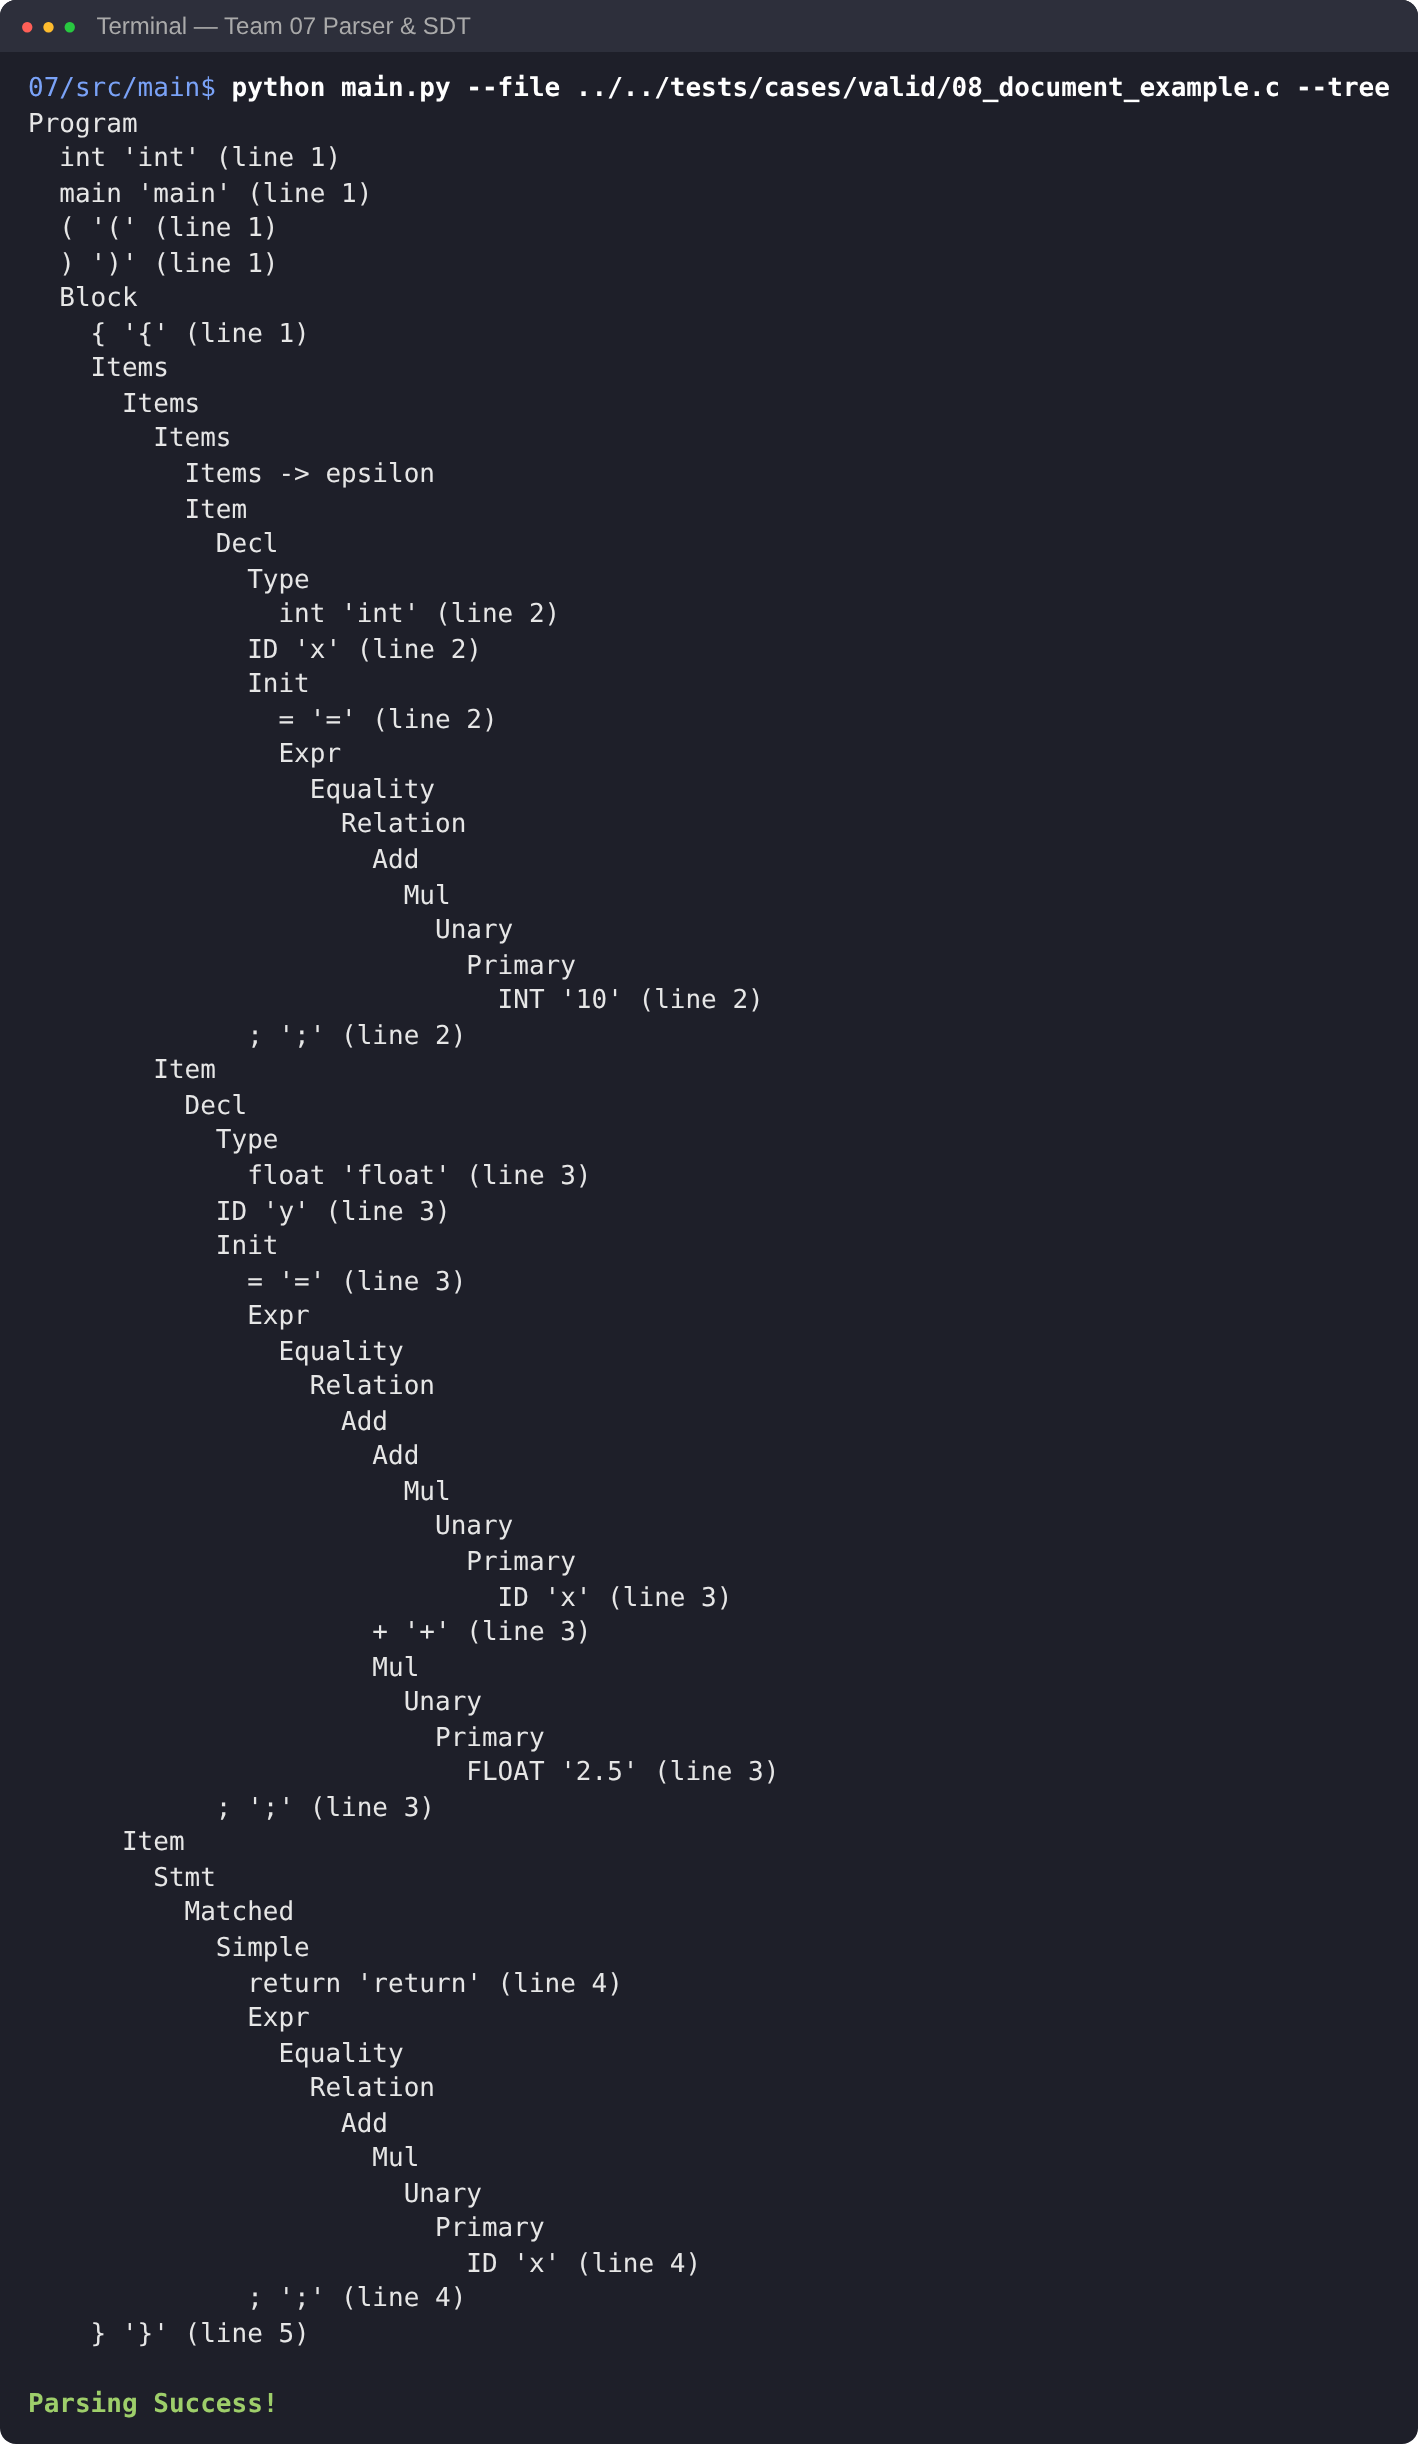
\includegraphics[width=0.58\linewidth]{shot_tree.png}
\caption{Parse tree printed with \texttt{-{}-tree} for
\texttt{valid/08\_document\_example.c}.}
\label{fig:tree}
\end{figure}

The tree also shows the effect of the grammar on precedence: in
\texttt{x + 2.5} the node \texttt{Add} has the children
\texttt{Add + Mul}; in the test \texttt{1 + 2 * 3} the multiplication is a
\texttt{Mul} node \emph{below} the \texttt{+}, so it is evaluated first.

% =====================================================================
\section{SDT rules}
% =====================================================================

A Syntax-Directed Translation associates semantic rules with the productions
of the grammar; the rules compute \emph{attributes} of the grammar symbols
\cite{aho2006}. The project uses mainly \emph{synthesized} attributes (they
flow from the children to the parent, the natural direction for a bottom-up
parser) and an environment (the symbol table) that is passed through the
tree in source order:

\begin{itemize}
  \item Expressions: \texttt{data\_type} (\texttt{int}, \texttt{float},
        \texttt{char} or \texttt{string}) and, for a simple literal,
        \texttt{literal\_lexeme}.
  \item \texttt{Type}: \texttt{data\_type}. \texttt{Init}: \texttt{present}
        and the type of its expression.
  \item \texttt{Block}: \texttt{scope\_id}.
\end{itemize}

Table~\ref{tab:sdt} lists the semantic action of every production.

{\small
\begin{longtable}{@{}p{1.6cm}p{4.3cm}p{9.2cm}@{}}
\caption{SDT rules per production.}\label{tab:sdt}\\
\toprule
\textbf{Prod.} & \textbf{Production} & \textbf{Semantic action}\\
\midrule
\endfirsthead
\toprule
\textbf{Prod.} & \textbf{Production} & \textbf{Semantic action}\\
\midrule
\endhead
0 & \texttt{Start -> Program} & ACCEPT; \texttt{Program} is the root of the tree. \\
1 & \texttt{Program -> int main ( ) Block} & \texttt{return\_type} $:=$ int; visit \texttt{Block}. \\
2 & \texttt{Block -> \{ Items \}} & Open a new scope (\texttt{scope\_id}), visit \texttt{Items}, close the scope. \\
3, 4 & \texttt{Items -> Items Item | $\varepsilon$} & Visit the items from left to right; the empty list is valid. \\
5, 6 & \texttt{Item -> Decl | Stmt} & Visit the child. \\
7 & \texttt{Decl -> Type ID Init ;} & If \texttt{ID} exists in the current scope: SEM001. Insert (\texttt{ID}, \texttt{Type.data\_type}) in the table. If \texttt{Init.present} and not assignable(\texttt{Type}, \texttt{Init}): SEM004. \\
8, 9, 10 & \texttt{Type -> int | float | char} & \texttt{Type.data\_type} $:=$ int / float / char. \\
11 & \texttt{Init -> = Expr} & \texttt{Init.present} $:=$ true; \texttt{Init.type} $:=$ \texttt{Expr.data\_type}. \\
12 & \texttt{Init -> $\varepsilon$} & \texttt{Init.present} $:=$ false. \\
13--16 & \texttt{Stmt}, \texttt{Matched} chains & Visit the child; a \texttt{Block} opens its own scope. \\
17, 19, 20 & \texttt{if ( Expr ) ...} & \texttt{Expr} must be numeric (else SEM006); visit the branches in source order. \\
18, 21 & \texttt{while ( Expr ) ...} & \texttt{Expr} must be numeric (else SEM006); check the body once (it is not executed). \\
22 & \texttt{Simple -> ID = Expr ;} & Look up \texttt{ID} (else SEM002); if not assignable(\texttt{ID.type}, \texttt{Expr.type}): SEM003. \\
23 & \texttt{Simple -> return Expr ;} & \texttt{Expr.type} must be assignable to int, the return type of \texttt{main} (else SEM007). \\
24 & \texttt{Simple -> ;} & No action. \\
25, 28, 33, 36, 40, 44 & pass-through (\texttt{Expr -> Equality}, \dots) & Copy \texttt{data\_type} (and \texttt{literal\_lexeme}) from the only child. \\
26, 27, 29--32 & \texttt{== != < <= > >=} & Both operands numeric (else SEM005); result int. \\
34, 35, 37, 38 & \texttt{+ - * /} & Both operands numeric (else SEM005); \texttt{char} is promoted to int; result float if any operand is float, int otherwise. \\
39 & \texttt{Mul -> Mul \% Unary} & Both operands char or int (else SEM005); result int. \\
41, 42 & \texttt{Unary -> + Unary | - Unary} & Operand numeric (else SEM005); result promote(type). \\
43 & \texttt{Unary -> ! Unary} & Operand numeric (else SEM005); result int. \\
45 & \texttt{Primary -> ID} & Look up the visible declaration (else SEM002); \texttt{data\_type} $:=$ its type. \\
46--49 & \texttt{Primary -> INT | FLOAT | CHAR | STRING} & \texttt{data\_type} $:=$ int / float / char / string; keep the lexeme. \\
50 & \texttt{Primary -> ( Expr )} & Copy the attributes of \texttt{Expr}. \\
\bottomrule
\end{longtable}
}

\subsection{Type policy}

For initialization, assignment and \texttt{return}, a value can be stored in
a type of the same or higher rank (\emph{widening}
\texttt{char -> int -> float}); \emph{narrowing} and strings are rejected
(Table~\ref{tab:assign}). This is a simplified, safer policy defined by the
team; it is stricter than ISO C, which allows implicit narrowing.

\begin{table}[!htbp]
\centering
\caption{assignable(destination, source).}
\label{tab:assign}
\begin{tabular}{@{}lcccc@{}}
\toprule
\textbf{Destination $\backslash$ source} & \textbf{char} & \textbf{int} & \textbf{float} & \textbf{string}\\
\midrule
char  & yes & no  & no  & no \\
int   & yes & yes & no  & no \\
float & yes & yes & yes & no \\
\bottomrule
\end{tabular}
\end{table}

% =====================================================================
\section{Semantic analysis}
% =====================================================================

The semantic analysis (\texttt{sdt.py}) runs \textbf{only after} the parser
accepts, on the complete tree. \texttt{SemanticAnalyzer} visits the tree in
source order and, at each node, executes the action of its production
(Table~\ref{tab:sdt}). It checks names, scopes and types; it does not execute
the program (it does not compute values or iterate loops). The first semantic
error stops the analysis and is reported with the line of the token
responsible for it (for example, the \tok{ID} of a duplicate declaration or
the keyword of a non-numeric condition). The errors are classified with the
codes of Table~\ref{tab:sem}.

\begin{table}[!htbp]
\centering
\caption{Semantic error codes.}
\label{tab:sem}
\small
\begin{tabularx}{\linewidth}{@{}lXl@{}}
\toprule
\textbf{Code} & \textbf{Error} & \textbf{Example} \\
\midrule
SEM001 & Duplicate declaration in the same scope & \texttt{int x; int x;} \\
SEM002 & Undeclared identifier (or out of scope)  & \texttt{y = 1;} \\
SEM003 & Incompatible assignment                  & \texttt{char c; c = c + 1;} \\
SEM004 & Incompatible initialization (invalid value for the declared type) & \texttt{int x = "hello";} \\
SEM005 & Invalid operand type for an operator      & \texttt{float f; int m = f \% 2;} \\
SEM006 & Non-numeric condition in \texttt{if}/\texttt{while} & \texttt{while ("a") ;} \\
SEM007 & \texttt{return} not compatible with int   & \texttt{return 2.5;} \\
\bottomrule
\end{tabularx}
\end{table}

\textbf{Why this is semantic and not syntactic.} A context-free grammar
cannot express ``a name must be declared before it is used'' or ``a name
cannot be declared twice in the same block'': these are context-sensitive
properties, since they relate two distant parts of the program. Types are
similar: \texttt{int x = "hello";} has exactly the same structure
(\texttt{Type ID = Expr ;}) as \texttt{int x = 10;}; only the attribute
\texttt{data\_type} of the expression distinguishes them. That is why these
checks belong to the SDT and why an input can produce
\ok{Parsing Success!} followed by \bad{SDT error}.

\subsection{Example: from the tree to the result}\label{sec:semex}

For the program

\noindent\begin{minipage}{\linewidth}
\begin{lstlisting}[style=ccode]
int main() {
    int x = 10;
    float y = x + 2.5;
    return x;
}
\end{lstlisting}
\end{minipage}

\begin{enumerate}
  \item p1 fixes the return type of \texttt{main} as int; p2 opens scope 0.
  \item Line 2, p7: \texttt{Type.data\_type} $=$ int; \texttt{x} is not in
        scope 0, so it is inserted. \texttt{Init} has the literal \texttt{10}
        (p46: int). assignable(int, int) holds.
  \item Line 3, p7: \texttt{y} is inserted as float. In \texttt{x + 2.5},
        p45 finds \texttt{x}: int; p47 gives float; p34 gives float because
        one operand is float. assignable(float, float) holds.
  \item Line 4, p23: \texttt{x} is int, assignable to the return type int.
  \item p2 closes scope 0. No rule failed: \ok{SDT Verified!}.
\end{enumerate}

% =====================================================================
\section{Symbol table}
% =====================================================================

The symbol table (\texttt{SymbolTable} in \texttt{sdt.py}) stores one record
per declaration: name, type, scope id, line and column of the declaration,
whether it has an initializer, and the initializer's type and lexeme. It
keeps a stack of active scopes:
\begin{itemize}
  \item every \texttt{Block} opens a new scope (the block of \texttt{main} is
        scope 0) and closes it when it ends;
  \item a lookup goes from the innermost active scope to the outermost one;
  \item declaring a name twice in the same scope is SEM001, but declaring it
        again in an inner scope is valid (\emph{shadowing});
  \item a name declared inside a block is not visible after the block closes
        (SEM002 if it is used);
  \item the records of closed scopes are kept, so the complete table can be
        shown at the end.
\end{itemize}
The variable is inserted \emph{before} its initializer is checked. This
choice is documented by the team: \texttt{int x = x;} is accepted, because the
analysis checks names and types but not definite initialization.

Figure~\ref{fig:symbols} shows the table for the example above. The
initializer of \texttt{y} is an expression, so no single lexeme is stored.

\begin{figure}[!htbp]
\centering
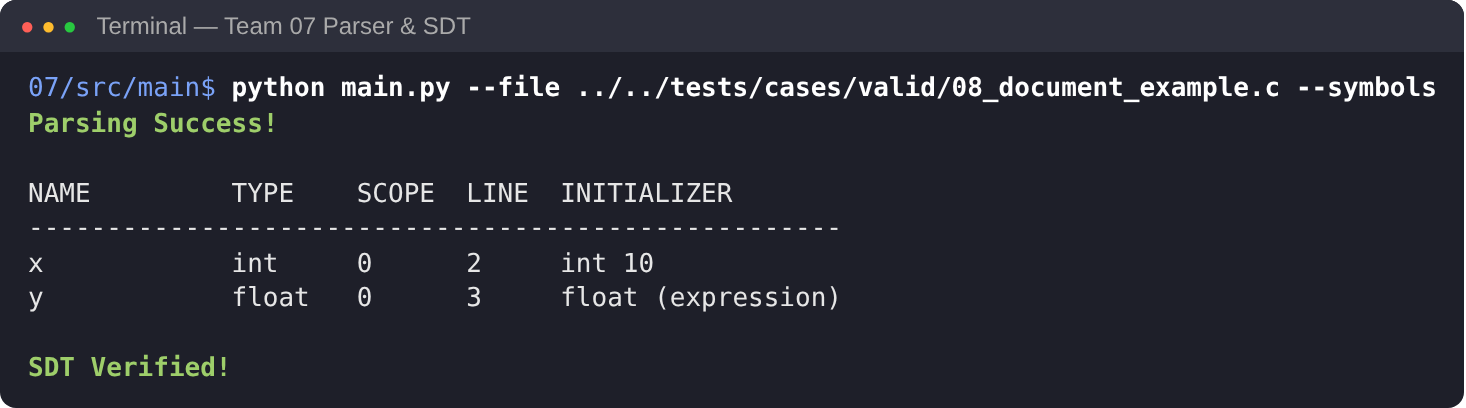
\includegraphics[width=0.75\linewidth]{shot_symbols.png}
\caption{Symbol table printed with \texttt{-{}-symbols}.}
\label{fig:symbols}
\end{figure}

For \texttt{valid/06\_scopes.c}, the table contains \texttt{x} (int, scope 0),
\texttt{x} (float, scope 1, the shadowing declaration) and \texttt{y} (int,
scope 2). The statement \texttt{return x;} after the inner block finds the
\texttt{x} of scope 0, of type int, and is therefore valid.

% =====================================================================
\section{Error handling}
% =====================================================================

Each phase stops the pipeline at its first error, and a later phase never
reports success if an earlier one failed. The order is:

\begin{enumerate}
  \item \textbf{Lexical error} $\rightarrow$ \bad{Lexical error in line n}.
        The lexer still scans the whole input and collects all errors, but
        the line reported is the first one. The parser is not executed,
        because the token stream is not valid.
  \item \textbf{Syntax error} $\rightarrow$ \bad{Parsing error in line n}.
        Produced by an empty ACTION cell. The SDT is not executed, since
        there is no complete tree on which to evaluate the rules. The line is
        the line of the unexpected token, or of the previous token if a
        \tok{;} was missing at the end of a line.
  \item \textbf{Semantic error} $\rightarrow$ \ok{Parsing Success!} followed
        by \bad{SDT error in line n}. Parsing succeeded (the tree exists), but
        an SDT rule failed. Only the first semantic error is reported.
\end{enumerate}

Internally, each error is an exception with additional details
(\texttt{ParseError.details()} names the expected terminals;
\texttt{SemanticError.details()} gives the code, column and lexeme), which
were used during development and in the tests.

% =====================================================================
\section{Test cases}
% =====================================================================

The project has two levels of tests, both automated with pytest \cite{pytest}:

\begin{itemize}
  \item \textbf{Unit tests} (208 tests) for each module: the lexer and its
        extensions, the token-to-terminal translation, the parser engine
        (shift/reduce/goto/accept on a small grammar, trace, error line,
        rejection of tables with conflicts, operator precedence in the tree; the
        shift/reduce trace with the team table, the parse tree of every valid
        case and the professor's example)
        and the SDT (compatibility matrix, promotion, scopes, shadowing,
        every error code, symbol table contents).
  \item \textbf{End-to-end cases} (\texttt{tests/cases/}): 42 C programs
        executed with the real program (\texttt{main.py -{}-file <case> -{}-sdt})
        and compared with a \texttt{.expected} file, in the four categories
        of the project: 10 valid, 12 syntax errors, 13 semantic errors and 7
        lexical errors. \texttt{test\_cases.py} runs them inside pytest
        (48 tests: the 42 cases plus checks of the case files), and \texttt{run\_cases.py} prints the comparison and
        regenerates \texttt{RESULTS.md} with expected and actual outputs.
\end{itemize}

\begin{figure}[!htbp]
\centering
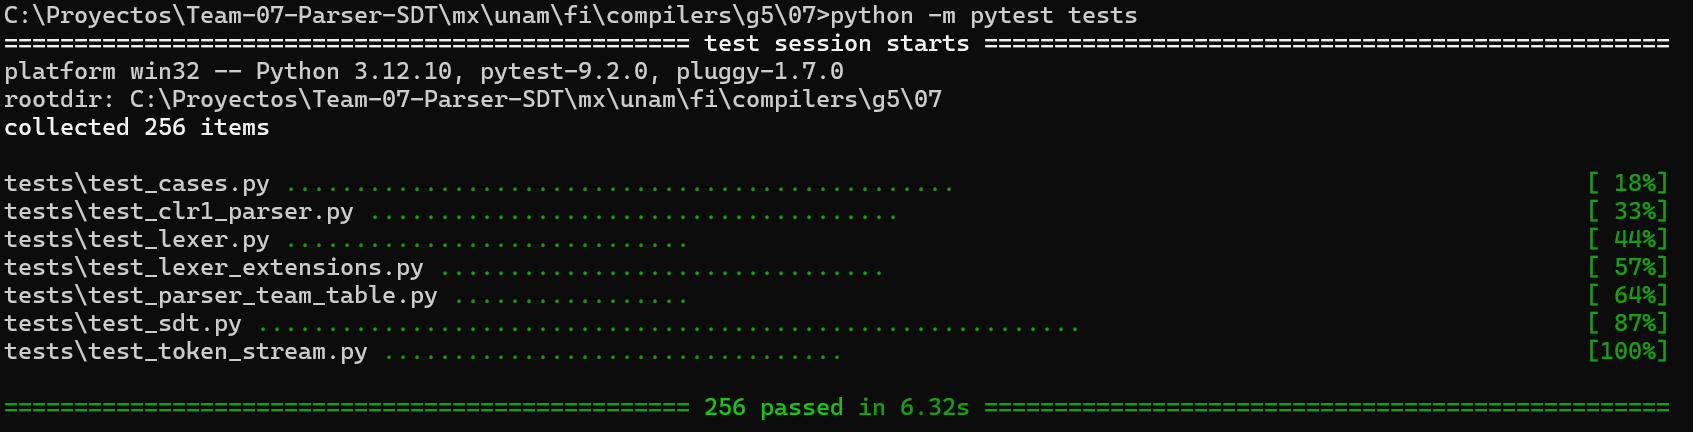
\includegraphics[width=0.95\linewidth]{shot_pytest_windows_256.png}
\caption{The complete test suite run on a team member's computer (Windows,
Python 3.12): 256 tests passed.}
\label{fig:pytest}
\end{figure}

% =====================================================================
\section{Results}
% =====================================================================

All 256 automated tests pass, and the 42 end-to-end cases produce exactly the
expected output (Figure~\ref{fig:cases}). This section shows representative
executions of each category and then justifies, case by case, why each input
produces its result.

\begin{figure}[!htbp]
\centering
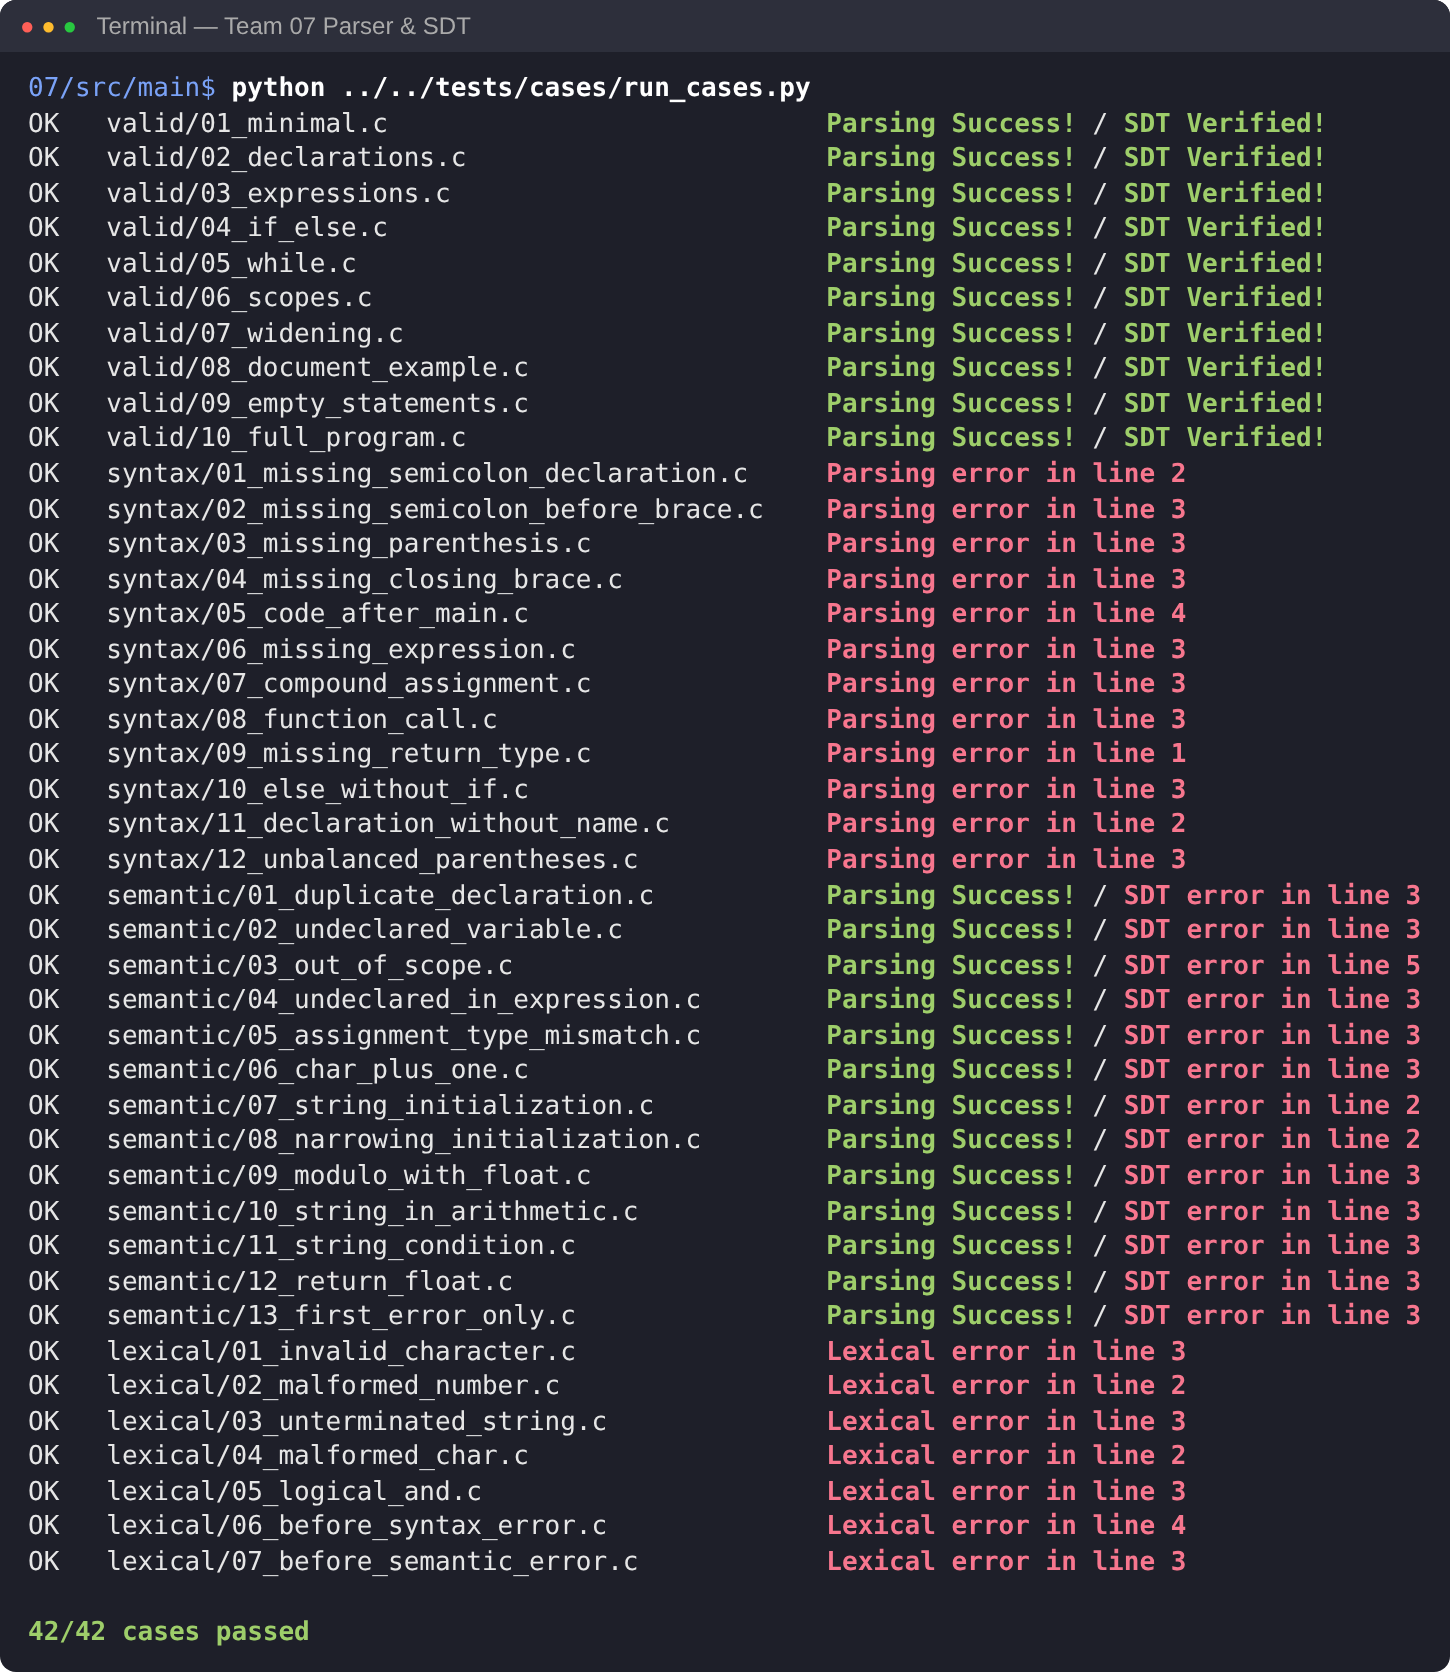
\includegraphics[width=0.8\linewidth]{shot_cases.png}
\caption{End-to-end cases: 42/42 produce the expected output.}
\label{fig:cases}
\end{figure}

\subsection{Representative executions}

Figures~\ref{fig:valid} to~\ref{fig:lexical} show one run of each category with the real program: valid inputs, syntax errors, semantic errors and lexical errors. Each run prints exactly the message predicted by the theory of the phase that stops the pipeline.

\begin{figure}[!htbp]
\centering
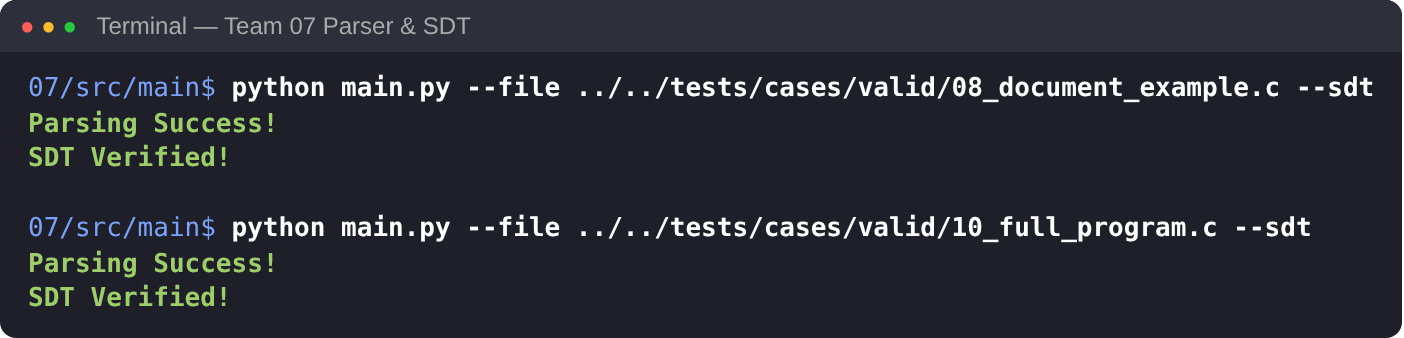
\includegraphics[width=0.66\linewidth]{shot_valid.png}
\caption{Valid input results.}
\label{fig:valid}
\end{figure}

\begin{figure}[!htbp]
\centering
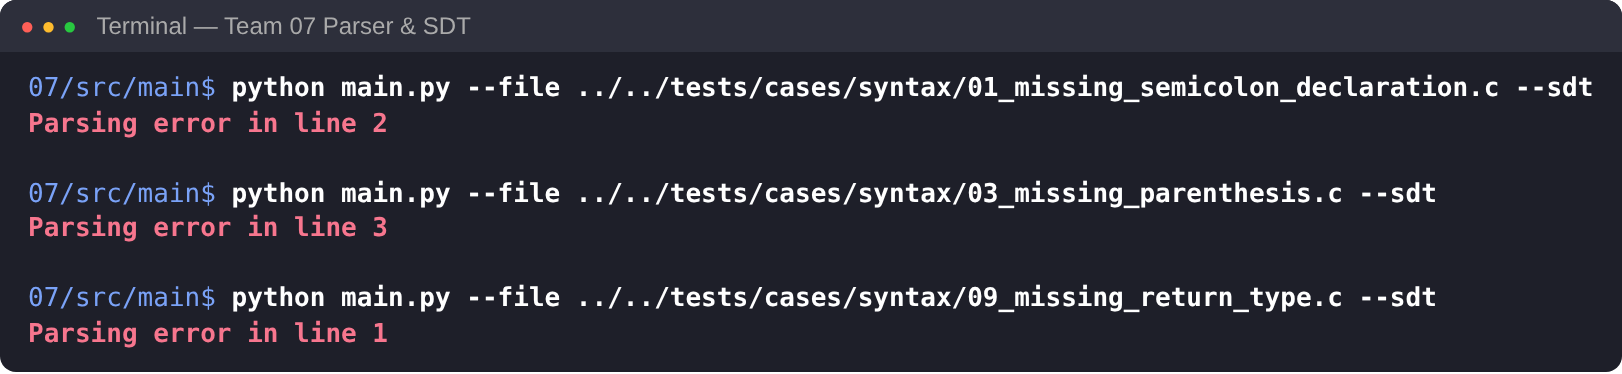
\includegraphics[width=0.78\linewidth]{shot_syntax.png}
\caption{Syntax error results.}
\label{fig:syntax}
\end{figure}

\begin{figure}[!htbp]
\centering
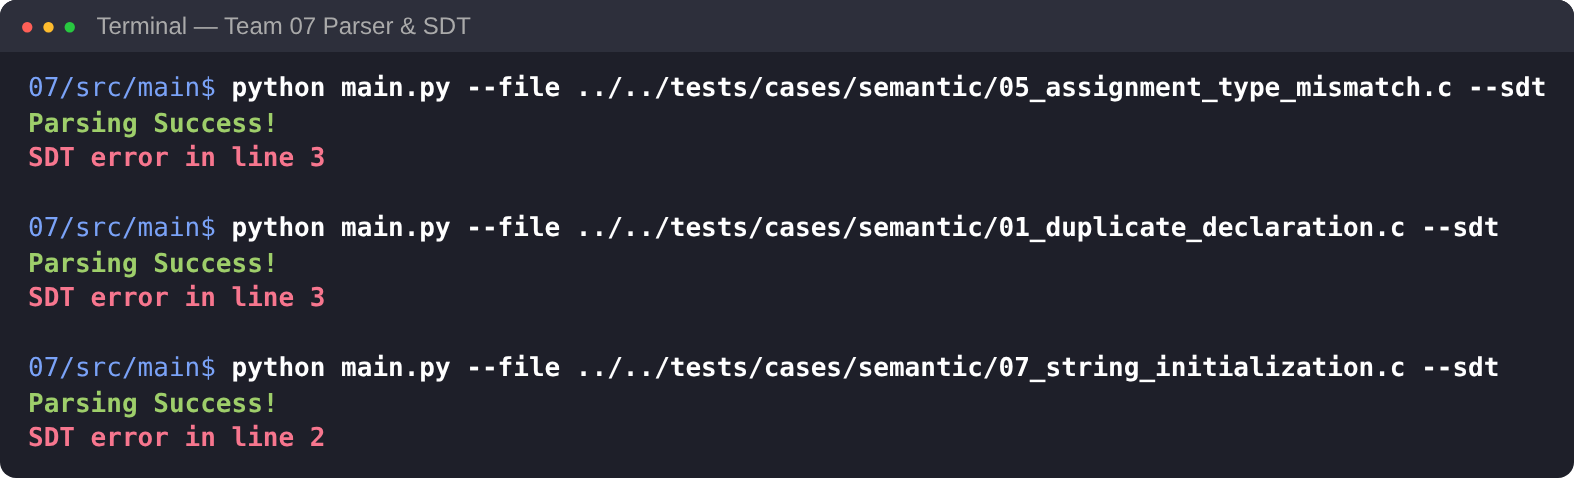
\includegraphics[width=0.78\linewidth]{shot_semantic.png}
\caption{Semantic error results (parsing succeeds, SDT fails).}
\label{fig:semantic}
\end{figure}

\begin{figure}[!htbp]
\centering
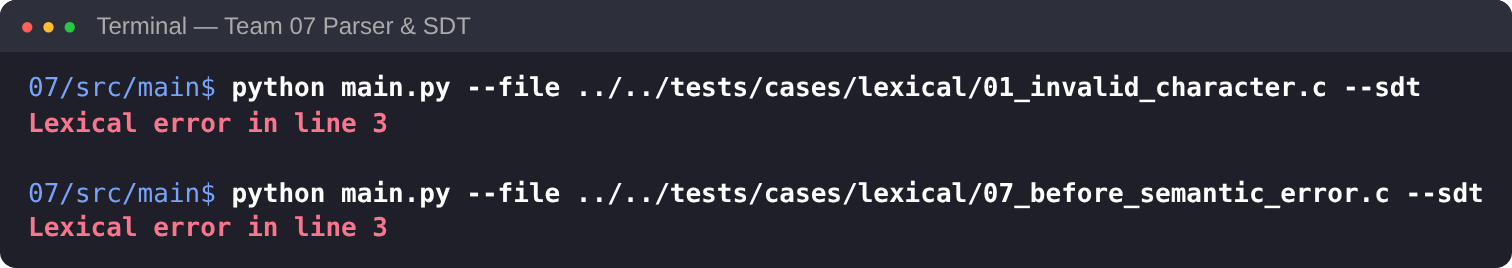
\includegraphics[width=0.7\linewidth]{shot_lexical.png}
\caption{Lexical error results: the parser is never executed.}
\label{fig:lexical}
\end{figure}

\subsection{Theoretical justification of each output}

\paragraph{\ok{Parsing Success!}} The CLR(1) driver reached the cell
ACTION[1, \$] $=$ accept. This only happens when the stack is \texttt{0 1},
that is, when the whole input has been reduced to \texttt{Program} and the
next symbol is the end of input. Since the table is the deterministic
automaton of the viable prefixes of the grammar, every shift and reduce taken
was valid, and the sequence of reductions is a rightmost derivation of the
input in reverse; hence the input belongs to $L(G)$ and its parse tree exists.

\paragraph{\bad{Parsing error in line n}} The driver reached an empty cell
ACTION[$s$, $a$]. Because the CLR(1) parser has the \emph{valid prefix
property}, it detects the error at the first token $a$ such that the prefix
read so far followed by $a$ cannot be the beginning of any sentence of the
grammar. Therefore no parse tree exists and the SDT cannot be evaluated.

\paragraph{\ok{SDT Verified!}} The parser accepted, and every semantic action
of every node of the tree was satisfied: each name was declared in a visible
scope and not duplicated in its own scope, and every attribute
\texttt{data\_type} satisfied the type rules of its production.

\paragraph{\bad{SDT error in line n}} The parser accepted (so it printed
\ok{Parsing Success!}), but at least one semantic action failed. The property
violated is context-sensitive or depends on attributes, so it cannot be
detected by the grammar; it is detected in the tree, after parsing.

\paragraph{\bad{Lexical error in line n}} The input contains a character
sequence that does not match any token pattern of the lexer. There is no
valid sequence of terminals, so the parser is not executed.

\subsection{Justification of each test case}

{\small
\begin{longtable}{@{}p{3.6cm}p{2.9cm}p{8.6cm}@{}}
\caption{Valid syntax and valid semantics.}\\
\toprule
\textbf{Case} & \textbf{Output} & \textbf{Why}\\
\midrule
\endfirsthead
\toprule
\textbf{Case} & \textbf{Output} & \textbf{Why}\\
\midrule
\endhead
01\_\allowbreak{}minimal & Success / Verified & \texttt{Items -> $\varepsilon$} (p4) gives an empty block; the derivation \texttt{Program -> int main ( ) \{ \}} exists and there is nothing to check. \\
02\_\allowbreak{}declarations & Success / Verified & Every declaration matches p7 with or without \texttt{Init}; each initializer has the same type as its variable. \\
03\_\allowbreak{}expressions & Success / Verified & Precedence levels p25--p50 generate every expression; all operands are numeric, \texttt{\%} only uses int, and the results (int or float) are assignable to their destinations. \\
04\_\allowbreak{}if\_\allowbreak{}else & Success / Verified & \texttt{Matched}/\texttt{Unmatched} attach the inner \texttt{else} to the nearest \texttt{if} without conflicts; conditions are int. \\
05\_\allowbreak{}while & Success / Verified & p18/p21 accept \texttt{while} with and without braces, nested; conditions are numeric comparisons. \\
06\_\allowbreak{}scopes & Success / Verified & Each \texttt{Block} opens a scope: the inner \texttt{float x} shadows the outer \texttt{int x} legally, and the outer variables remain visible in nested blocks. \\
07\_\allowbreak{}widening & Success / Verified & Only widening conversions (\texttt{char -> int -> float}); \texttt{\textquotesingle{}b\textquotesingle{} + 1} is int and is stored in a float. \\
08\_\allowbreak{}document\_\allowbreak{}example & Success / Verified & Example of Section~\ref{sec:semex}: \texttt{x + 2.5} is float, \texttt{return x} is int. \\
09\_\allowbreak{}empty\_\allowbreak{}statements & Success / Verified & \texttt{Simple -> ;} (p24) and empty blocks are valid statements; \texttt{0} and \texttt{1} are numeric conditions. \\
10\_\allowbreak{}full\_\allowbreak{}program & Success / Verified & Combines all the constructs; \texttt{suma / 5.0} is float, assigned to the float \texttt{promedio}. \\
\bottomrule
\end{longtable}

\begin{longtable}{@{}p{3.6cm}p{2.9cm}p{8.6cm}@{}}
\caption{Invalid syntax.}\\
\toprule
\textbf{Case} & \textbf{Output} & \textbf{Why}\\
\midrule
\endfirsthead
\toprule
\textbf{Case} & \textbf{Output} & \textbf{Why}\\
\midrule
\endhead
01\_\allowbreak{}missing\_\allowbreak{}semicolon\_\allowbreak{}declaration & Parsing error, line 2 & After \texttt{int x = 5} the parser expects an operator or \tok{;}; \tok{return} (line 3) has no action. Inserting \tok{;} would make \tok{return} valid, so the error belongs to line 2. \\
02\_\allowbreak{}missing\_\allowbreak{}semicolon\_\allowbreak{}before\_\allowbreak{}brace & Parsing error, line 3 & \texttt{return x} followed by \tok{\}}: p23 requires \tok{;}. The \tok{\}} is on line 4, but the missing \tok{;} is on line 3. \\
03\_\allowbreak{}missing\_\allowbreak{}parenthesis & Parsing error, line 3 & In \texttt{if (a > 0 \{}, after an expression inside \texttt{if (} only an operator or \tok{)} is valid; \tok{\{} has no action. \\
04\_\allowbreak{}missing\_\allowbreak{}closing\_\allowbreak{}brace & Parsing error, line 3 & The input ends (\tok{\$}) while \texttt{Block} still needs \tok{\}}; ACTION[$s$, \$] is empty. \tok{\$} is placed after the last token, on line 3. \\
05\_\allowbreak{}code\_\allowbreak{}after\_\allowbreak{}main & Parsing error, line 4 & After \texttt{Program} is complete only \tok{\$} is valid; \tok{int} on line 4 has no action. Only one \texttt{main} function is a \texttt{Program}. \\
06\_\allowbreak{}missing\_\allowbreak{}expression & Parsing error, line 3 & After \texttt{a =} an \texttt{Expr} must start; \tok{;} is not in FIRST(Expr). \\
07\_\allowbreak{}compound\_\allowbreak{}assignment & Parsing error, line 3 & \texttt{+=} is tokenized as \tok{+} \tok{=}; after \tok{ID} at the start of a statement only \tok{=} is valid. \\
08\_\allowbreak{}function\_\allowbreak{}call & Parsing error, line 3 & Calls are not in the grammar: after \tok{ID} at the start of a statement, \tok{(} has no action. \\
09\_\allowbreak{}missing\_\allowbreak{}return\_\allowbreak{}type & Parsing error, line 1 & ACTION[0, $t$] is defined only for \tok{int}; the first terminal is \tok{main}. \\
10\_\allowbreak{}else\_\allowbreak{}without\_\allowbreak{}if & Parsing error, line 3 & \tok{else} is not in FIRST(Item) and no open \texttt{if} can take it. \\
11\_\allowbreak{}declaration\_\allowbreak{}without\_\allowbreak{}name & Parsing error, line 2 & In $I_{22}$ (\texttt{Type -> int .}) the only lookahead is \tok{ID}; \tok{=} has no action. \\
12\_\allowbreak{}unbalanced\_\allowbreak{}parentheses & Parsing error, line 3 & The second \tok{)} has no matching \tok{(}: after a complete expression only \tok{;} or an operator is valid. \\
\bottomrule
\end{longtable}

\begin{longtable}{@{}p{3.6cm}p{2.9cm}p{8.6cm}@{}}
\caption{Valid syntax but invalid semantics (all print \ok{Parsing Success!} first).}\\
\toprule
\textbf{Case} & \textbf{Output} & \textbf{Why}\\
\midrule
\endfirsthead
\toprule
\textbf{Case} & \textbf{Output} & \textbf{Why}\\
\midrule
\endhead
01\_\allowbreak{}duplicate\_\allowbreak{}declaration & SDT error, line 3 & SEM001: \texttt{x} already exists in scope 0. The grammar allows any sequence of declarations; uniqueness is context-sensitive. \\
02\_\allowbreak{}undeclared\_\allowbreak{}variable & SDT error, line 3 & SEM002: \texttt{y = ...} is a valid p22, but \texttt{y} is not in any active scope. \\
03\_\allowbreak{}out\_\allowbreak{}of\_\allowbreak{}scope & SDT error, line 5 & SEM002: \texttt{z} was declared in scope 1, which was closed with its block. \\
04\_\allowbreak{}undeclared\_\allowbreak{}in\_\allowbreak{}expression & SDT error, line 3 & SEM002: p45 cannot find \texttt{c}. \\
05\_\allowbreak{}assignment\_\allowbreak{}type\_\allowbreak{}mismatch & SDT error, line 3 & SEM003: \texttt{2.5} is float; assignable(int, float) is false (narrowing). \\
06\_\allowbreak{}char\_\allowbreak{}plus\_\allowbreak{}one & SDT error, line 3 & SEM003: \texttt{c + 1} promotes char to int; int cannot be stored in char. \\
07\_\allowbreak{}string\_\allowbreak{}initialization & SDT error, line 2 & SEM004: \texttt{"hello"} is string; strings are not assignable to any declarable type. \\
08\_\allowbreak{}narrowing\_\allowbreak{}initialization & SDT error, line 2 & SEM004: \texttt{65} is int; int $\to$ char is narrowing under the team policy. \\
09\_\allowbreak{}modulo\_\allowbreak{}with\_\allowbreak{}float & SDT error, line 3 & SEM005: p39 requires char or int operands; \texttt{f} is float. \\
10\_\allowbreak{}string\_\allowbreak{}in\_\allowbreak{}arithmetic & SDT error, line 3 & SEM005: p34 requires numeric operands; \texttt{"dos"} is string. \\
11\_\allowbreak{}string\_\allowbreak{}condition & SDT error, line 3 & SEM006: the condition of \texttt{while} has type string, not numeric. \\
12\_\allowbreak{}return\_\allowbreak{}float & SDT error, line 3 & SEM007: \texttt{f} is float; \texttt{main} returns int. \\
13\_\allowbreak{}first\_\allowbreak{}error\_\allowbreak{}only & SDT error, line 3 & Two errors (SEM002 in line 3, SEM001 in line 4); the analysis visits in source order and stops at the first. \\
\bottomrule
\end{longtable}

\begin{longtable}{@{}p{3.6cm}p{2.9cm}p{8.6cm}@{}}
\caption{Lexical errors (the parser is never executed).}\\
\toprule
\textbf{Case} & \textbf{Output} & \textbf{Why}\\
\midrule
\endfirsthead
\toprule
\textbf{Case} & \textbf{Output} & \textbf{Why}\\
\midrule
\endhead
01\_\allowbreak{}invalid\_\allowbreak{}character & Lexical error, line 3 & \texttt{@} does not belong to any token pattern. \\
02\_\allowbreak{}malformed\_\allowbreak{}number & Lexical error, line 2 & \texttt{12abc} is a single malformed token (longest match), not a constant followed by an identifier. \\
03\_\allowbreak{}unterminated\_\allowbreak{}string & Lexical error, line 3 & The string has no closing quote before the end of the line. \\
04\_\allowbreak{}malformed\_\allowbreak{}char & Lexical error, line 2 & A character literal must contain exactly one character; \texttt{\textquotesingle{}ab\textquotesingle{}} has two. \\
05\_\allowbreak{}logical\_\allowbreak{}and & Lexical error, line 3 & \texttt{\&} is not an operator of the subset, so \texttt{\&\&} is a lexical error. \\
06\_\allowbreak{}before\_\allowbreak{}syntax\_\allowbreak{}error & Lexical error, line 4 & There is a syntax error in line 2, but the lexer runs first and \texttt{\#} invalidates the token stream: the parser never runs. \\
07\_\allowbreak{}before\_\allowbreak{}semantic\_\allowbreak{}error & Lexical error, line 3 & There is a semantic error in line 2 (\texttt{y} undeclared), but \texttt{\$} in line 3 stops the process before the parser and the SDT. \\
\bottomrule
\end{longtable}
}

% =====================================================================
\FloatBarrier
\section{Conclusions}
% =====================================================================

The project fulfills the requirements of the statement: the input is the
token stream of the team's lexer; the grammar is defined on exactly those
tokens; a bottom-up CLR(1) parser builds the parse tree; and SDT rules verify
it. The program distinguishes the four results required, including the case
in which parsing succeeds but the SDT fails, and reports the line of each
error. Everything was built from the theory seen in class, without parser
generators.

Building the canonical collection showed in practice why CLR(1) is more
powerful than SLR(1): the lookaheads computed with FIRST($\beta a$) place each
reduction only where it is valid in its context, and states with the same
core but different lookaheads (such as $I_9$ and $I_{122}$) remain separate.
As a result, a grammar written naturally, with left recursion,
$\varepsilon$-productions, six precedence levels and the \emph{dangling else}
solved by \texttt{Matched}/\texttt{Unmatched}, has a table of 161 states with
no conflicts.

The separation between syntax and semantics was also clear in the results.
The grammar decides the \emph{structure} of the program, and the SDT decides
the properties that depend on context: declarations, scopes and types. The
semantic test cases are syntactically correct programs that differ from
valid ones only in an attribute or in a declaration located elsewhere, which
is exactly why they must be detected after parsing.

Finally, keeping the grammar and the table as data shared by the documents,
the code and the tests made the model and the implementation consistent,
and the 256 automated tests give evidence that every output of the program
has the theoretical cause described in this report.

\newpage
% =====================================================================
\begin{thebibliography}{9}
\addcontentsline{toc}{section}{References}
% =====================================================================

\bibitem{aho2006}
A.~V. Aho, M.~S. Lam, R. Sethi, and J.~D. Ullman, \emph{Compilers:
Principles, Techniques, and Tools}, 2nd~ed. Boston, MA, USA: Pearson
Addison-Wesley, 2006.

\bibitem{hopcroft2007}
J.~E. Hopcroft, R. Motwani, and J.~D. Ullman, \emph{Introduction to Automata
Theory, Languages, and Computation}, 3rd~ed. Boston, MA, USA: Pearson
Addison-Wesley, 2007.

\bibitem{knuth1965}
D.~E. Knuth, ``On the translation of languages from left to right,''
\emph{Information and Control}, vol.~8, no.~6, pp.~607--639, 1965.

\bibitem{parserpdf}
Compilers, Group~5, ``Parser \& SDT,'' project statement, Faculty of
Engineering, National Autonomous University of Mexico, Mexico City, Mexico,
2026.

\bibitem{md}
B. Y\'a\~nez Barajas (Team~07, Model Designer), ``Gram\'atica y tokens,
Colecci\'on can\'onica LR(1), Tabla CLR(1) ACTION/GOTO, Reglas SDT y tabla de
s\'imbolos,'' project documents, \texttt{docs/model-designer/}, 2026.

\bibitem{pytest}
pytest-dev, ``pytest documentation.'' Accessed: Nov.~8, 2026. [Online].
Available: \url{https://docs.pytest.org/}

\bibitem{lexerrepo}
Team~07, ``Team-07: Lexical analyzer,'' GitHub repository, 2026. [Online].
Available: \url{https://github.com/HansZuniga/Team-07}

\bibitem{repo}
Team~07, ``Team-07-Parser-SDT: Parser and syntax-directed translation,''
GitHub repository, 2026. [Online]. Available:
\url{https://github.com/HansZuniga/Team-07-Parser-SDT}

\end{thebibliography}

\end{document}
